\documentclass[11pt,a4paper,titlepage,openany]{report}

% --- Pacchetti Fondamentali di Sistema e Lingua ---
\usepackage[utf8]{inputenc}
\usepackage[T1]{fontenc}
\usepackage[italian]{babel}
\usepackage{lmodern}
\usepackage[a4paper,top=2.8cm,bottom=2.8cm,left=3.0cm,right=2.8cm]{geometry}

% --- Matematica e Simboli ---
\usepackage{amsmath,amssymb,amsfonts,mathtools,bm}

% --- Grafica e Tabelle ---
\usepackage{graphicx}
\graphicspath{{figure/}{../figure/}}
\usepackage{booktabs}
\usepackage{tabularx}
\usepackage{array}
\newcolumntype{L}{>{\raggedright\arraybackslash}X}
\usepackage{multirow}
\usepackage{longtable}
\usepackage{float}
\usepackage{caption}
\usepackage{subcaption}

% --- Tipografia e Stile ---
\usepackage{microtype}
\usepackage{xcolor}
\usepackage{fancyhdr}
\usepackage{cite}
\usepackage{url}
\usepackage{hyperref}

% --- Palette Cromatica Accademica ---
\definecolor{primaryblue}{RGB}{27, 79, 114}     % #1b4f72
\definecolor{accentblue}{RGB}{41, 128, 185}     % #2980b9
\definecolor{darkcharcoal}{RGB}{44, 62, 80}     % #2c3e50
\definecolor{darkgray}{RGB}{60, 60, 60}
\definecolor{lightgray}{RGB}{245, 247, 248}

% --- Configurazione Collegamenti Ipertestuali ---
\hypersetup{
    colorlinks=true,
    linkcolor=primaryblue,
    citecolor=accentblue,
    urlcolor=accentblue,
    pdftitle={Rilevamento di POI senza Bounding Box Annotate: Pseudo-Label da DINOv3 (WSOL) e Distillazione in YOLOv8},
    pdfauthor={Giovanni Piccinini},
    pdfsubject={Deep Learning - Core Models and Methods - UNICT-VEDI POI}
}

% --- Formattazione Didascalie ---
\captionsetup{
    font=small,
    labelfont={bf,color=primaryblue},
    format=hang,
    margin=10pt
}

% --- Intestazioni e Piè di Pagina ---
\pagestyle{fancy}
\fancyhf{}
\fancyhead[L]{\small\color{darkcharcoal}\nouppercase{\leftmark}}
\fancyhead[R]{\small\color{darkcharcoal}\thepage}
\renewcommand{\headrulewidth}{0.5pt}
\renewcommand{\footrulewidth}{0pt}

% Stile pulito per inizio capitoli
\fancypagestyle{plain}{
    \fancyhf{}
    \fancyfoot[C]{\small\color{darkcharcoal}\thepage}
    \renewcommand{\headrulewidth}{0pt}
}

% Formattazione elegante dei titoli di capitolo (standard LaTeX)
\makeatletter
\def\@makechapterhead#1{%
  \vspace*{20\p@}%
  {\parindent \z@ \raggedright \normalfont
    \ifnum \c@secnumdepth >\m@ne
      \large\bfseries\color{accentblue} CAPITOLO \thechapter
      \par\nobreak
      \vskip 6\p@
    \fi
    \interlinepenalty\@M
    \Huge \bfseries\color{primaryblue} #1\par\nobreak
    \vskip 8\p@
    {\color{accentblue}\hrule height 1.2pt}
    \vskip 20\p@
  }}
\def\@makeschapterhead#1{%
  \vspace*{20\p@}%
  {\parindent \z@ \raggedright
    \normalfont
    \interlinepenalty\@M
    \Huge \bfseries\color{primaryblue} #1\par\nobreak
    \vskip 8\p@
    {\color{accentblue}\hrule height 1.2pt}
    \vskip 20\p@
  }}
\makeatother

\begin{document}

% ==============================================================================
% FRONTESPIZIO ACCADEMICO
% ==============================================================================
\begin{titlepage}
    \centering
    \vspace*{0.5cm}
    
    {\Large\textsc{Università degli Studi di Catania}}\\[0.3cm]
    {\large\textsc{Dipartimento di Matematica e Informatica}}\\[0.2cm]
    {\normalsize Corso di Laurea Magistrale in Informatica LM-18}\\[2.5cm]
    
    {\huge\bfseries\color{primaryblue} Rilevamento di POI senza Bounding Box Annotate}\\[0.5cm]
    {\LARGE\bfseries\color{accentblue} Pseudo-Label da DINOv3 (WSOL) e Distillazione in YOLOv8}\\[0.6cm]
    {\large Studio di Sample Efficiency e Capacity Retention sul Dataset Monumentale UNICT-VEDI}\\[3.0cm]
    
    \begin{minipage}[t]{0.45\textwidth}
        \flushleft
        \textbf{\color{darkcharcoal}Studente:}\\[0.15cm]
        Giovanni Piccinini\\[0.1cm]
        Matricola 1000097151
    \end{minipage}
    \hfill
    \begin{minipage}[t]{0.50\textwidth}
        \flushright
        \textbf{\color{darkcharcoal}Corso:}\\[0.15cm]
        Deep Learning - Core Models and Methods\\[0.3cm]
        \textbf{\color{darkcharcoal}Docenti:}\\[0.15cm]
        Prof. Giovanni Maria Farinella\\[0.1cm]
        Prof. Francesco Ragusa
    \end{minipage}
    
    \vfill
    {\small\color{darkcharcoal} Anno Accademico 2025/2026}
\end{titlepage}

% ==============================================================================
% SOMMARIO E INDICI
% ==============================================================================
\pagenumbering{roman}

\cleardoublepage
\phantomsection
\addcontentsline{toc}{chapter}{Sommario}
\chapter*{Sommario}

L'annotazione manuale di riquadri di delimitazione (\textit{bounding box}) per l'object detection richiede tempo e risorse considerevoli, in particolare nei domini specialistici come i beni culturali. In questo lavoro si esamina il paradigma della \textit{Weakly-Supervised Object Localization} (WSOL) applicato al dataset egocentrico UNICT-VEDI POI, che raccoglie 57 classi di elementi monumentali nel Monastero dei Benedettini di Catania.

Sfruttando le feature di auto-segmentazione del modello DINOv3 ViT-S/16 con testa lineare (\textit{linear probing}), è stata definita una procedura basata su Linear-CAM per ricavare pseudo-annotazioni spaziali a partire dalle sole etichette di classe dell'immagine. Le etichette così generate servono ad addestrare il rilevatore compatto YOLOv8n, senza impiegare coordinate cartesiane supervisionate nel processo di apprendimento.

Per quantificare il risparmio di annotazione, è stato impostato un confronto di \textit{sample efficiency} rispetto a baseline supervisionate addestrate su quote progressive ($1\% \dots 100\%$) del ground truth con tre repliche stocastiche. Il modello distillato ottiene il $37.39\%$ di mAP@50, prestazione equivalente all'$1.43\%$ di dati etichettati a mano e pari al $61.79\%$ della capacità del rilevatore supervisionato al $100\%$. L'analisi per scala dimensionale evidenzia una ritenzione del $63.60\%$ nel Tier Macro (26 classi di taglia intermedia non degeneri) e dell'$84.14\%$ nel Tier Full-Frame. L'esame dei fallimenti nel Tier Tiny ($0.00\%$ mAP@50) mostra inoltre che l'errore sistematico non deriva dalla risoluzione spaziale delle patch, ma dal bias di contesto e dall'\textit{attribution leakage}: i massimi di attivazione del classificatore scivolano sulle strutture murarie contigue anziché sul piccolo reperto da localizzare.


\tableofcontents
\cleardoublepage

\listoffigures
\cleardoublepage

\listoftables
\cleardoublepage

% ==============================================================================
% CAPITOLI DELLA RELAZIONE
% ==============================================================================
\pagenumbering{arabic}

\chapter{Introduzione e Definizione del Problema}
\label{chap:introduzione}

\section{Contesto Applicativo: Visione Egocentrica nei Beni Culturali}
\label{sec:intro_contesto}
La \textit{First-Person Vision} (FPV), o visione egocentrica, cattura flussi visivi tramite dispositivi indossabili (\textit{wearable cameras} o visori) dal punto di vista prospettico del visitatore. Nei contesti museali o monumentali, individuare in tempo reale i punti di interesse (POI) osservati dall'utente (\textit{attended objects}) è il passo preliminare per costruire sistemi interattivi di guida e fruizione culturale.

Come benchmark di riferimento viene adottato il dataset UNICT-VEDI POI~\cite{ragusa2019egocentric}, acquisito nel complesso del Monastero dei Benedettini di San Nicolò l'Arena a Catania. Il corpus raccoglie 57 classi di elementi storici e architettonici (dipinti, affreschi, portali e ambienti) ripresi durante percorsi di visita continui.

\section{L'Asimmetria dei Costi di Annotazione}
\label{sec:intro_asimmetria}
I modelli supervisionati di object detection richiedono grandi quantità di riquadri di delimitazione (\textit{bounding box}) tracciati a mano. Nei beni culturali questo comporta un netto sbilanciamento nei costi di etichettatura:
\begin{itemize}
    \item \textbf{Supervisione a livello di immagine (\textit{image-level})}: annotare la presenza del POI nella scena richiede circa $1 - 2$ secondi per fotogramma ed è spesso ricavabile da log di visita o sensori di prossimità.
    \item \textbf{Supervisione geometrica (\textit{bounding box})}: delimitare i contorni di opere asimmetriche o parzialmente occluse richiede $20 - 30$ secondi per fotogramma, diventando presto insostenibile su raccolte video di decine di migliaia di fotogrammi.
\end{itemize}
Questo divario di costi motiva l'interesse per la \textit{Weakly-Supervised Object Localization} (WSOL)~\cite{choe2020evaluating,zhang2018adversarial,bilgi2021weakly}, che mira a ricavare la posizione 2D degli oggetti partendo dalle sole etichette di presenza nell'immagine.

\section{Domanda di Ricerca}
\label{sec:intro_domanda}
La letteratura su WSOL si concentra quasi sempre su metriche isolate di localizzazione (come mAP@50 o MaxBoxAcc). Sul piano pratico ed economico resta però aperta una domanda diretta:
\begin{quote}
    \centering
    \textit{<<A quale frazione di dati annotati manualmente con bounding box equivale un sistema di localizzazione addestrato senza alcuna annotazione geometrica supervisionata?>>}
\end{quote}
Nel presente lavoro si misura la \textit{sample efficiency} della supervisione debole, determinando a quale quota percentuale di ground truth manuale corrisponda il modello distillato e quanta frazione della capacità del rilevatore pienamente supervisionato (l'oracolo al $100\%$) venga effettivamente preservata.

\section{Panoramica della Pipeline Proposta}
\label{sec:intro_pipeline}
Per rispondere alla domanda, la sperimentazione è stata organizzata in cinque fasi:
\begin{enumerate}
    \item \textbf{Modello teacher (DINOv3)}: addestramento di una testa lineare su backbone Vision Transformer congelato (ViT-S/16)~\cite{caron2021emerging,oquab2023dinov2,simeoni2025dinov3}, mantenendo intatte le feature di auto-segmentazione spaziale.
    \item \textbf{Attribuzione spaziale (WSOL)}: estrazione delle mappe di salienza con Linear-CAM e confronto comparativo con \textit{DINO Self-Attention}, \textit{Eigen-CAM}~\cite{muhammad2020eigen} e \textit{Grad-CAM}~\cite{selvaraju2017grad}.
    \item \textbf{Generazione di pseudo-label}: trasformazione deterministica delle heatmap in riquadri in formato YOLO tramite sogliatura proporzionale, apertura morfologica ed estrazione del poligono sul picco di attivazione.
    \item \textbf{Distillazione dello studente (YOLOv8n)}: addestramento del rilevatore leggero YOLOv8n ($3.2\text{M}$ parametri)~\cite{jocher2023ultralytics} sull'insieme di immagini etichettato automaticamente dal teacher.
    \item \textbf{Valutazione di sample efficiency}: confronto dello studente distillato con 19 baseline supervisionate addestrate su 7 quote di ground truth ($1\% \dots 100\%$) su 3 seed casuali, valutate sul test set ufficiale.
\end{enumerate}

\section{Organizzazione del Documento}
\label{sec:intro_struttura}
Il documento è organizzato come segue: il Capitolo~\ref{chap:dataset} descrive il dataset VEDI, la pulizia dei dati e la suddivisione in tier dimensionali; il Capitolo~\ref{chap:architettura} presenta l'architettura DINOv3 e la derivazione di Linear-CAM; il Capitolo~\ref{chap:training_classificatore} riporta i risultati di classificazione e la distribuzione degli errori nelle sale; il Capitolo~\ref{chap:wsol} confronta i 4 metodi CAM; il Capitolo~\ref{chap:distillazione} illustra la distillazione in YOLOv8n; il Capitolo~\ref{chap:sample_efficiency} descrive il protocollo di sample efficiency; il Capitolo~\ref{chap:risultati} analizza il punto di pareggio, la ritenzione di capacità e il bias contestuale sulle classi Tiny; i Capitoli~\ref{chap:limiti} e~\ref{chap:conclusioni} discutono i limiti riscontrati, le conclusioni e le possibili estensioni. Le Appendici~\ref{chap:appendice_iperparametri}--\ref{chap:appendice_note_tecniche} contengono i parametri completi, la tassonomia delle classi e le note di riproducibilità.

\chapter{Il Dataset UNICT-VEDI POI e Sanitizzazione delle Annotazioni}
\label{chap:dataset}

\section{Struttura e Origine del Dataset UNICT-VEDI POI}
\label{sec:dataset_struttura}

\subsection{Origine scientifica e contesto applicativo}
Il benchmark utilizzato è il dataset UNICT-VEDI POI~\cite{ragusa2019egocentric}, curato dall'IPLab dell'Università di Catania all'interno del progetto VEDI. I dati appartengono all'ambito della \textit{First-Person Vision} (FPV) nei beni culturali: i video sono stati acquisiti tramite videocamere indossate da visitatori all'interno del Monastero dei Benedettini di San Nicolò l'Arena a Catania.

Il compito applicativo consiste nell'individuare automaticamente i punti di interesse (POI) osservati dall'utente (\textit{attended objects}). Il corpus comprende affreschi, tele, sculture, portali ed elementi architettonici, con le caratteristiche sintetiche riportate nella Tabella~\ref{tab:dataset_proprieta}.

\begin{table}[htbp]
\centering
\small
\begin{tabularx}{\textwidth}{lL}
\toprule
\textbf{Proprietà del Dataset} & \textbf{Valore / Dettaglio Operativo} \\
\midrule
\textbf{Sito monumentale} & Monastero dei Benedettini di San Nicolò l'Arena (Catania) \\
\textbf{Tipologia dati} & Fotogrammi da video egocentrici ($1216 \times 684$ pixel) \\
\textbf{Numero di classi POI} & 57 classi distribuite su 9 macro-ambienti storici \\
\textbf{Volume Training Set} & $67.050$ immagini (organizzate per cartella di classe) \\
\textbf{Volume Test Set} & $5.462$ immagini (distribuite su 7 sessioni continue di visita) \\
\textbf{Formato annotazioni} & Coordinate bounding box normalizzate ($x_c, y_c, w, h$) \\
\bottomrule
\end{tabularx}
\caption{Specifiche strutturali del dataset egocentrico UNICT-VEDI POI.}
\label{tab:dataset_proprieta}
\end{table}

\subsection{Tassonomia delle classi e articolazione spaziale}
I 57 POI sono distribuiti nei 9 macro-ambienti del monastero (Tabella~\ref{tab:tassonomia_aree}). L'elenco integrale classe per classe con le aree medie è riportato in Appendice~\ref{chap:appendice_classi}.

\begin{table}[htbp]
\centering
\small
\begin{tabularx}{\textwidth}{l c L}
\toprule
\textbf{Macro-Ambiente Storico} & \textbf{POI ($N$)} & \textbf{Esempi Rappresentativi} \\
\midrule
\textbf{1. Ingresso Monumentale} & 1 & Ingresso \\
\textbf{2. Scalone Monumentale} & 2 & Rampa S. Nicola, Rampa S. Benedetto \\
\textbf{3. Chiostro e Corridoi} & 11 & Chiostro Levante, Affresco, Traccia Portone, Corridoi \\
\textbf{4. Cantoria e Chiesa} & 3 & Quadro, Pavimento Orig. Altare, Balcone Chiesa \\
\textbf{5. Antirefettorio e Museo} & 10 & Portali, Cupola, S. Agata, S. Scolastica, Busto Vaccarini \\
\textbf{6. Coro di Notte e Aula} & 9 & Quadro Mazzarino, Bassorilievi Mancanti, Lavamani, Poltrone \\
\textbf{7. Refettorio Piccolo} & 7 & Edicola, Pavimenti A/B, Passavivande, Scala, Sala Metereologica \\
\textbf{8. Cucine e Sotterranei} & 11 & Doccione, Cucine, Ghiacciaia, Cisterna, Busto Tacchini \\
\textbf{9. Giardino dei Novizi} & 3 & Nicchia e Pavimento, Tracce Palestra, Pergolato \\
\midrule
\textbf{Totale Complesso} & \textbf{57} & Tassonomia completa dettagliata in Appendice~\ref{chap:appendice_classi} \\
\bottomrule
\end{tabularx}
\caption{Distribuzione delle 57 classi di POI nei 9 macro-ambienti monumentali.}
\label{tab:tassonomia_aree}
\end{table}

\subsection{Organizzazione tra Training e Test Set}
L'organizzazione tra addestramento e test presenta una differenza strutturale importante:
\begin{itemize}
    \item \textbf{Training set ($67.050$ immagini)}: le immagini sono raggruppate in 57 cartelle, una per ciascuna classe di POI.
    \item \textbf{Test set ($5.462$ immagini)}: i fotogrammi provengono da 7 sessioni continue di visita a passo d'uomo (\texttt{Test1}--\texttt{Test7}). Di questi, $3.673$ fotogrammi presentano annotazioni di ground truth con coordinate geometriche; i rimanenti corrispondono a momenti di passaggio tra ambienti privi di soggetti catalogati.
\end{itemize}

\section{Sanitizzazione delle Annotazioni del Dataset}
\label{sec:dataset_sanitizzazione}
L'analisi preliminare dei file di etichetta in formato YOLO ($[x_c, y_c, w, h] \in [0, 1]^4$) ha evidenziato anomalie corrette tramite tre passaggi di pulizia:
\begin{enumerate}
    \item \textbf{Normalizzazione delle coordinate}: i riquadri salvati con coordinate assolute in pixel (valori maggiori di $1.5$) sono stati ricondotti all'intervallo $[0, 1]$ dividendo per le dimensioni d'origine del fotogramma ($W=1216, H=684$).
    \item \textbf{Troncamento ai bordi (\textit{clamping})}: le coordinate esterne all'immagine sono state tagliate sull'intervallo $[0.0, 1.0]$, ponendo $x_{\min}^{\text{clamp}} = \max(0.0, \min(1.0, x_{\min}))$ e analogamente per gli altri tre vertici.
    \item \textbf{Rimozione dei riquadri degeneri}: sono state rimosse le annotazioni con larghezza o altezza inferiori a $\epsilon = 10^{-3}$, per evitare divergenze numeriche nel calcolo dell'Intersection over Union.
\end{enumerate}

\subsection{Trattamento dei fotogrammi privi di bounding box: Convenzione Full-Frame}
Nel set di addestramento, $3.106$ fotogrammi (circa il $4.6\%$ del totale) sono privi di file di etichetta. Seguendo la documentazione ufficiale del dataset rilasciata dagli autori:
\begin{quote}
    \textit{<<Some folders have not the two *.csv files, in this case for each related RGB frame you have to consider a bounding box which contains the whole frame.>>}
\end{quote}
è stata assegnata a queste immagini la classe associata alla cartella e un riquadro esteso all'intero fotogramma ($[x_c = 0.5, y_c = 0.5, w = 1.0, h = 1.0]$). Questa scelta modella le situazioni in cui l'ambiente o la parete monumentale occupa completamente la vista dell'utente.

\section{Analisi dell'Area Media per Classe e Definizione dei Tier Dimensionali}
\label{sec:dataset_tiers}

\subsection{Motivazione metodologica}
Le dimensioni apparenti dei soggetti nel dataset variano da piccoli dettagli scultorei a lunghi corridoi. Valutare i modelli solo tramite la metrica mAP aggregata nasconderebbe differenze marcate nel comportamento del Vision Transformer a scale spaziali diverse.

\paragraph{Nota metodologica sui Tier.}
La ripartizione in fasce dimensionali (tier) non appartiene alla specifica originaria del dataset VEDI: è stata introdotta in questo studio per analizzare il rendimento dei metodi in funzione dell'ingombro relativo dell'oggetto.

\subsection{Formulazione e distribuzione nei 4 tier}
I tier sono calcolati a livello di classe mediante l'area media normalizzata $\bar{A}_c$ occupata dal riquadro di ground truth su tutte le occorrenze:
\begin{equation}
    \bar{A}_c = \frac{1}{N_c} \sum_{i=1}^{N_c} (w_{c,i} \cdot h_{c,i}) \in [0.0, 1.0]
\end{equation}
Le 57 classi sono state quindi ripartite in quattro fasce (Tabella~\ref{tab:distribuzione_tiers}).

\begin{table}[htbp]
\centering
\footnotesize
\setlength{\tabcolsep}{3.5pt}
\begin{tabularx}{\textwidth}{lcccccX}
\toprule
\textbf{Tier} & \textbf{Soglia ($\bar{A}_c$)} & \textbf{Classi} & \textbf{Quota} & \textbf{Area Media} & \textbf{Range} & \textbf{Esempi} \\
\midrule
\textbf{Tiny} & $\le 0.10$ & \textbf{4} & $7.0\%$ & \textbf{4.97\%} & $3.1\% - 7.2\%$ & Bassorilievi, S. Agata \\
\textbf{Small} & $0.10 - 0.30$ & \textbf{3} & $5.3\%$ & \textbf{26.27\%} & $21.9\% - 29.7\%$ & Quadro Mazzarino, Lavamani \\
\textbf{Macro} & $0.30 - 0.80$ & \textbf{27} & $47.4\%$ & \textbf{61.19\%} & $31.5\% - 78.6\%$ & Portali, affreschi, altari \\
\textbf{Full-Frame} & $\ge 0.80$ & \textbf{23} & $40.3\%$ & \textbf{93.09\%} & $81.3\% - 99.8\%$ & Corridoi, scalinate, sale \\
\midrule
\textbf{Totale} & — & \textbf{57} & $100\%$ & \textbf{70.75\%} & $3.1\% - 99.8\%$ & — \\
\bottomrule
\end{tabularx}
\caption{Segmentazione delle 57 classi del dataset UNICT-VEDI POI nei quattro tier dimensionali analitici (in Area Media e Range sono riportate le quote percentuali dell'inquadratura).}
\label{tab:distribuzione_tiers}
\end{table}

\subsection{Caratteristiche dei singoli tier}
\begin{enumerate}
    \item \textbf{Tier Tiny (4 classi, area $\bar{A}_c \le 0.10$)}: elementi circoscritti (Bassorilievi, S.~Agata, S.~Scolastica, Cupola). Costituiscono il caso più critico per la localizzazione debole, sia per la discretizzazione spaziale a patch, sia per la predominanza visiva della muratura circostante.
    \item \textbf{Tier Small (3 classi, $0.10 < \bar{A}_c < 0.30$)}: soggetti delimitati (Quadro Mazzarino, Lavamani, Busto Tacchini). Con lo sfondo che copre tra il $70\%$ e il $90\%$ della scena, le mappe di attivazione tendono a disperdersi sui muri d'appoggio.
    \item \textbf{Tier Macro (27 classi, $0.30 \le \bar{A}_c < 0.80$)}: il gruppo più numeroso ($47.4\%$). Raccoglie portali, affreschi e scalinate in cui il soggetto riempie buona parte dell'inquadratura ma conserva contorni netti rispetto all'ambiente.
    \item \textbf{Tier Full-Frame (23 classi, $\bar{A}_c \ge 0.80$)}: corridoi e sale ampie con copertura media del $93.1\%$. In questa fascia il compito geometrico coincide nei fatti con la classificazione dell'ambiente, dato che il riquadro corretto coincide quasi per intero con l'immagine.
\end{enumerate}

\chapter{DINOv3 e Architettura del Classificatore}
\label{chap:architettura}

\section{Vision Transformer e Paradigma DINO}
\label{sec:arch_vit}

\subsection{Fondamenti del Vision Transformer}
L'architettura \textit{Vision Transformer} (ViT)~\cite{dosovitskiy2020image} adatta il meccanismo di auto-attenzione (\textit{self-attention})~\cite{vaswani2017attention} alla visione artificiale. Un'immagine d'ingresso $I \in \mathbb{R}^{H \times W \times C}$ viene suddivisa in $N = (H \cdot W) / P^2$ patch bidimensionali disgiunte di lato $P$. Ciascuna patch viene proiettata linearmente in uno spazio latente di dimensione $D$. Alla sequenza risultante è anteposto un token apprendibile ($\mathbf{z}_{\text{CLS}} \in \mathbb{R}^D$), deputato a raccogliere la semantica globale, ed è sommato un vettore di posizione $\mathbf{E}_{\text{pos}} \in \mathbb{R}^{(N+1) \times D}$:
\begin{equation}
    \mathbf{z}_0 = \left[ \mathbf{z}_{\text{CLS}}; \, \mathbf{x}_p^1 \mathbf{E}; \, \dots; \, \mathbf{x}_p^N \mathbf{E} \right] + \mathbf{E}_{\text{pos}}
\end{equation}
La sequenza attraversa $L$ blocchi di \textit{Transformer Encoder}, composti da strati alternati di \textit{Multi-Head Self-Attention} (MHSA) e \textit{Multi-Layer Perceptron} (MLP), preceduti da normalizzazione di strato (\textit{LayerNorm}):
\begin{align}
    \mathbf{z}'_\ell &= \text{MHSA}(\text{LN}(\mathbf{z}_{\ell-1})) + \mathbf{z}_{\ell-1}, \quad \ell = 1, \dots, L \\
    \mathbf{z}_\ell &= \text{MLP}(\text{LN}(\mathbf{z}'_\ell)) + \mathbf{z}'_\ell
\end{align}
In ciascuna delle $h$ teste, l'attenzione opera con dimensione $d_k = D / h$ mediante prodotto scalare scalato:
\begin{equation}
    \text{Attention}(\mathbf{Q}, \mathbf{K}, \mathbf{V}) = \text{Softmax}\left( \frac{\mathbf{Q} \mathbf{K}^\top}{\sqrt{d_k}} \right) \mathbf{V}
\end{equation}
Questo meccanismo offre un campo recettivo globale fin dal primo strato, correlando elementi visivi anche a grande distanza nell'immagine.

\subsection{Pre-addestramento auto-supervisionato in DINOv3}
Privo dell'inductive bias convoluzionale, ViT richiede ampi volumi di dati per apprendere rappresentazioni visive robuste. I modelli DINO~\cite{caron2021emerging,oquab2023dinov2,simeoni2025dinov3} superano questo vincolo mediante auto-supervisione su larga scala: in DINOv3 l'addestramento impiega il corpus LVD-1689M (circa 1.7 miliardi di immagini).

\begin{figure}[htbp]
\centering
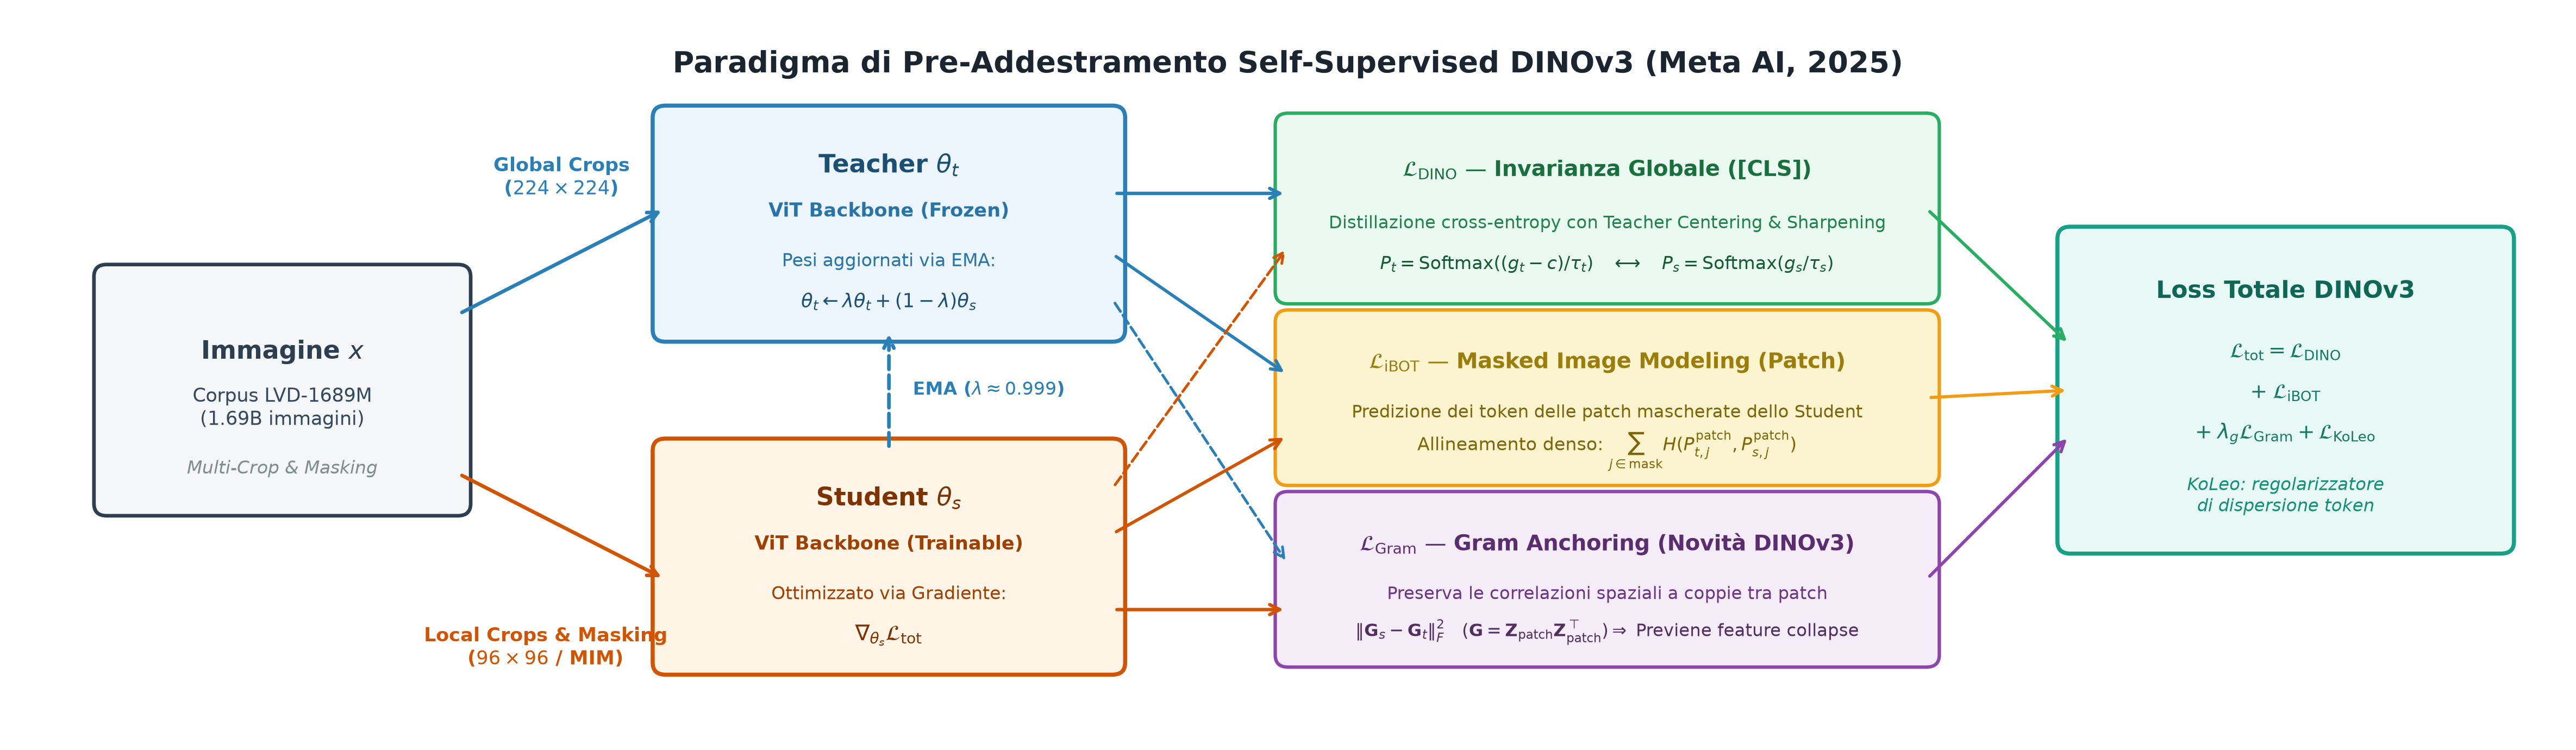
\includegraphics[width=0.92\textwidth]{figure/schema_dino_pretraining.png}
\caption{Architettura di pre-addestramento auto-supervisionato DINOv3~\cite{simeoni2025dinov3}. La rete Student è ottimizzata su obiettivi congiunti ($\mathcal{L}_{\mathrm{DINO}}$, $\mathcal{L}_{\mathrm{iBOT}}$, $\mathcal{L}_{\mathrm{Gram}}$, $\mathcal{L}_{\mathrm{KoLeo}}$); la rete Teacher è aggiornata tramite EMA, guidando la distillazione a livello globale ($[\mathrm{CLS}]$) e denso (patch).}
\label{fig:dino_pretraining}
\end{figure}

Il framework si basa su una distillazione tra due reti omologhe (Figura~\ref{fig:dino_pretraining}): una rete \textbf{Student} con parametri $\theta_s$, ottimizzata via gradiente, e una rete \textbf{Teacher} con parametri $\theta_t$, aggiornata per media mobile esponenziale (EMA):
\begin{equation}
    \theta_t \leftarrow \lambda \theta_t + (1 - \lambda) \theta_s, \quad \lambda \in [0.99, 1.0]
\end{equation}
DINOv3 combina tre funzioni di costo principali e un termine di regolarizzazione:
\begin{enumerate}
    \item \textbf{Loss DINO} ($\mathcal{L}_{\mathrm{DINO}}$): cross-entropy sui token $[\mathrm{CLS}]$ tra ritagli globali e locali. L'uscita del Teacher è stabilizzata tramite \textit{centering} (sottrazione della media empirica dei logit) e \textit{sharpening} (temperatura ridotta sul Softmax), inducendo invarianza alle trasformazioni geometriche.
    \item \textbf{Loss iBOT} ($\mathcal{L}_{\mathrm{iBOT}}$): masked image modeling a livello di patch token; lo Student predice le patch mascherate allineandosi alle rappresentazioni dense non mascherate del Teacher.
    \item \textbf{Gram Anchoring} ($\mathcal{L}_{\mathrm{Gram}}$): vincolo caratterizzante di DINOv3 che allinea le matrici di Gram (correlazioni a coppie tra patch) tra Student e Teacher, prevenendo il collasso delle feature dense durante l'ottimizzazione prolungata su scala miliardaria.
    \item \textbf{Regolarizzatore KoLeo} ($\mathcal{L}_{\mathrm{KoLeo}}$): massimizza l'entropia differenziale, distribuendo uniformemente i vettori latenti nello spazio unitario.
\end{enumerate}
Questo schema integrato consente ai token dell'ultimo strato di catturare confini semantici e separare naturalmente l'oggetto in primo piano dallo sfondo, costituendo la premessa per la localizzazione debolmente supervisionata tramite mappe di attivazione.

\section{Backbone ViT-S/16 e Testa Lineare}
\label{sec:arch_linear_probing}

\subsection{Configurazione del backbone}
Nel presente lavoro viene impiegato il checkpoint ViT-S/16 pre-addestrato. I parametri architetturali sono riassunti nella Tabella~\ref{tab:iperparametri_vits16}.

\begin{table}[htbp]
\centering
\small
\begin{tabularx}{\textwidth}{lcX}
\toprule
\textbf{Iperparametro} & \textbf{Valore} & \textbf{Descrizione Operativa} \\
\midrule
\textbf{Dimensione latente ($D$)} & $384$ & Dimensione del vettore di embedding di ciascun token \\
\textbf{Numero di strati ($L$)} & $12$ & Blocchi sequenziali di Transformer Encoder \\
\textbf{Teste di attenzione ($h$)} & $6$ & Numero di teste nel modulo Multi-Head Self-Attention \\
\textbf{Dimensione per testa ($d_k$)} & $64$ & Spazio di proiezione di ciascuna testa ($384 / 6$) \\
\textbf{Dimensione patch ($P$)} & $16$ & Risoluzione spaziale di ciascuna patch ($16 \times 16$ px) \\
\textbf{Numero di parametri} & $\approx 22\text{ M}$ & Complessità parametrica complessiva del backbone \\
\bottomrule
\end{tabularx}
\caption{Parametri architetturali del backbone DINOv3 ViT-S/16.}
\label{tab:iperparametri_vits16}
\end{table}

\subsection{Linear Probing con backbone congelato}
Per preservare lo spazio latente pre-addestrato ed evitare il \textit{catastrophic forgetting}, il backbone è mantenuto a pesi congelati ($\nabla_{\theta_{\text{backbone}}} \mathcal{L} = 0$).
Sul token globale $\mathbf{z}_{\text{CLS}}^{(L)} \in \mathbb{R}^{384}$ dell'ultimo strato è innestata una testa di classificazione lineare preceduta da Dropout ($p = 0.3$):
\begin{equation}
    \hat{\mathbf{y}} = \mathbf{W} \cdot \text{Dropout}(\mathbf{z}_{\text{CLS}}^{(L)}) + \mathbf{b}
\end{equation}
dove $\mathbf{W} \in \mathbb{R}^{57 \times 384}$ mappa i descrittori latenti sulle $57$ classi del dataset e $\mathbf{b} \in \mathbb{R}^{57}$ è il vettore di bias.

\begin{figure}[htbp]
\centering
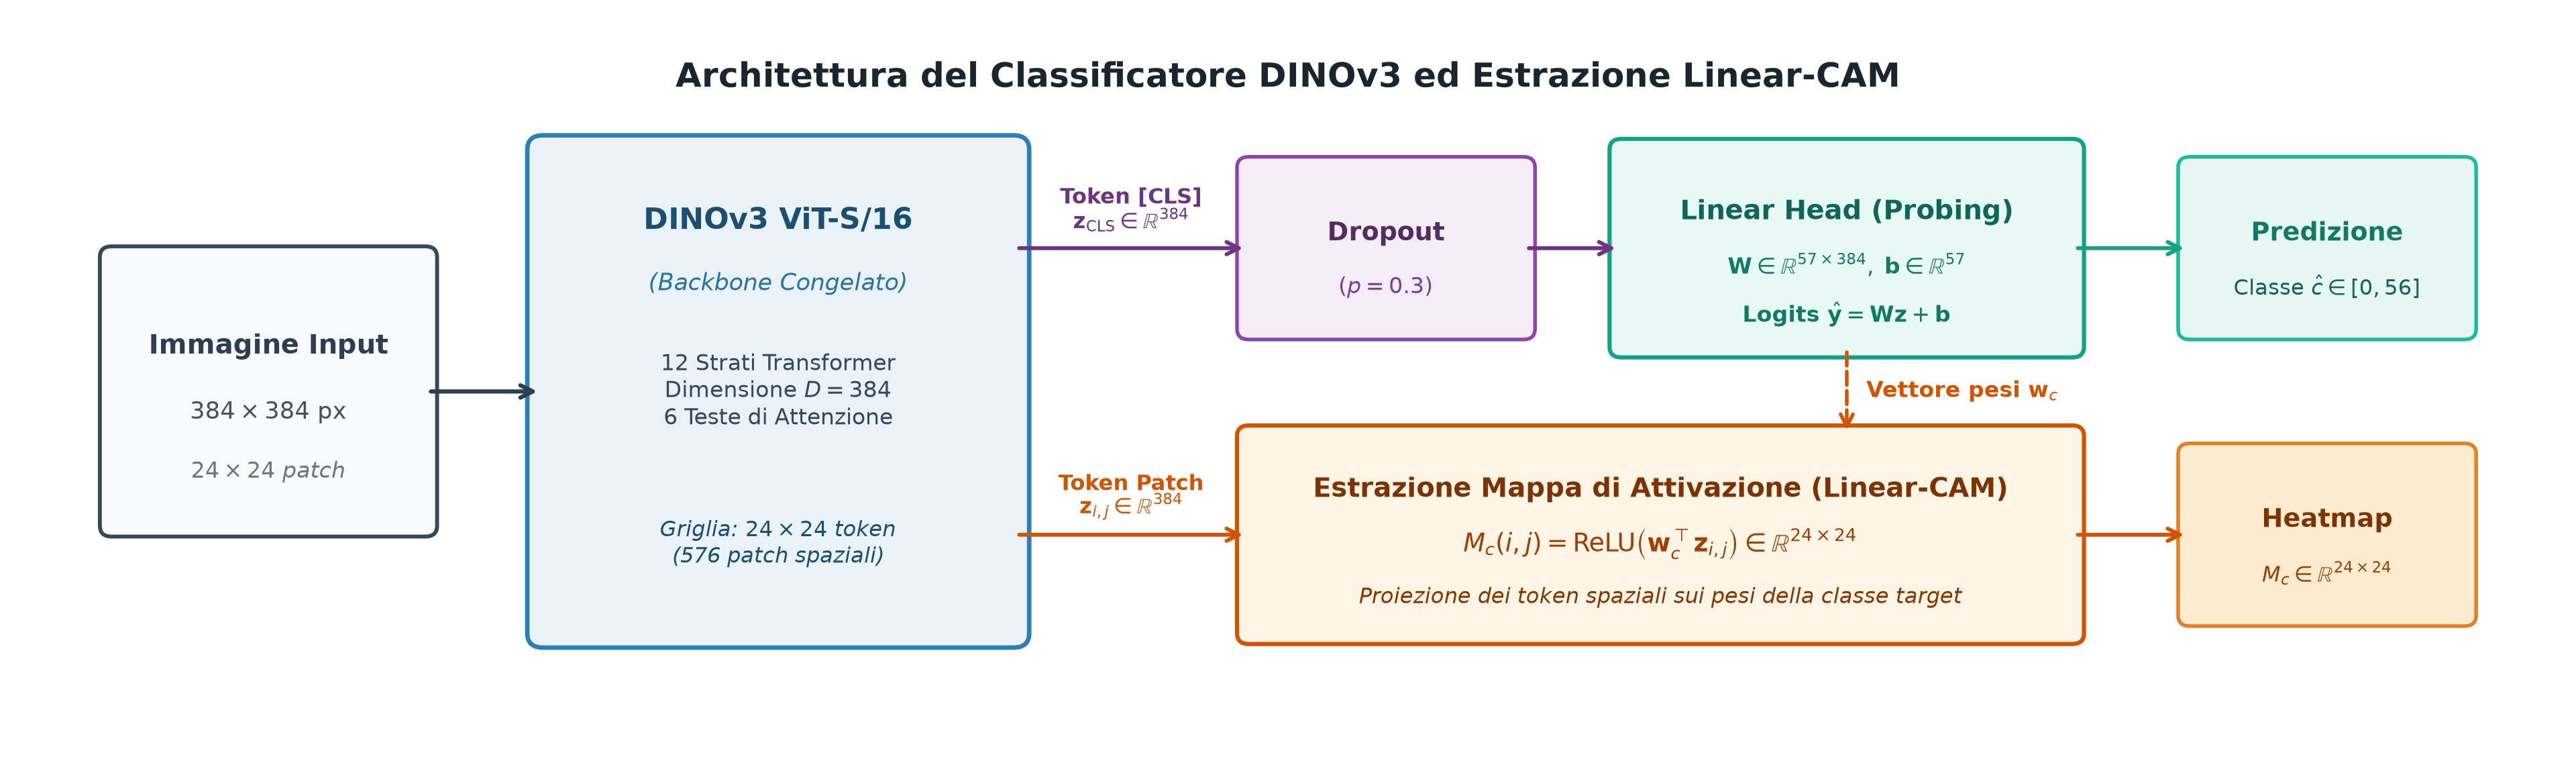
\includegraphics[width=0.88\textwidth]{figure/architettura_classificatore.png}
\caption{Flusso computazionale del classificatore: il backbone ViT-S/16 congelato fornisce sia il token $[\text{CLS}]$ per la predizione di classe (ramo superiore), sia i token di patch impiegati per l'attribuzione Linear-CAM (ramo inferiore).}
\label{fig:architettura_classificatore}
\end{figure}

La linearità della testa fa sì che ciascuna riga $\mathbf{w}_c \in \mathbb{R}^{384}$ della matrice $\mathbf{W}$ corrisponda alla direzione prototipo per la classe $c$. Questa proprietà consente di valutare direttamente l'attivazione locale proiettando $\mathbf{w}_c$ sui singoli token di patch.

\section{Discretizzazione in Patch e Risoluzione Spaziale}
\label{sec:arch_risoluzione}
A risoluzione d'ingresso $H = W = 384$ pixel e lato patch $P = 16$, l'immagine viene suddivisa in una griglia regolare $24 \times 24$, per un totale di $N = 576$ token spaziali oltre al token $[\text{CLS}]$. Ogni cella $(i, j)$ corrisponde a un'area di $16 \times 16$ pixel.
Nei soggetti a scala ridotta (Tier Tiny, area relativa $3\% - 7\%$), il target copre appena $17-40$ celle; in tale intervallo, l'interpolazione continua e la sogliatura operano in prossimità del limite di risoluzione della griglia, aumentando la sensibilità a dispersioni di salienza sullo sfondo.

\section{Metodi di Attribuzione per la Localizzazione Debole (WSOL)}
\label{sec:arch_wsol_cenni}
La combinazione tra i token spaziali di DINOv3 e la testa lineare permette di calcolare quattro mappe di salienza continua $M_c(i, j) \in \mathbb{R}^{24 \times 24}$ per la classe predetta $c$:
\begin{enumerate}
    \item \textbf{Linear-CAM (pesi di classe)}~\cite{zhou2016learning}:
    \begin{equation}
        M_{\text{Linear}}(i, j) = \text{ReLU}\left( \mathbf{w}_c^\top \mathbf{z}_{i, j} \right)
    \end{equation}
    dove $\mathbf{w}_c$ è il vettore dei pesi della classe $c$ e $\mathbf{z}_{i, j}$ è l'embedding del token in $(i, j)$.
    \item \textbf{DINO Self-Attention}:
    \begin{equation}
        M_{\text{Attn}}(i, j) = \frac{1}{h} \sum_{k=1}^h \mathbf{A}_{k}^{(L)}[\text{CLS}, \, (i, j)]
    \end{equation}
    ovvero l'attenzione del token $[\text{CLS}]$ verso i token di patch all'ultimo strato.
    \item \textbf{Eigen-CAM (decomposizione spettrale)}~\cite{muhammad2020eigen}:
    \begin{equation}
        M_{\text{Eigen}}(i, j) = \mathbf{V}_1^\top \mathbf{z}_{i, j}
    \end{equation}
    proiettando le feature spaziali sul primo autovettore principale $\mathbf{V}_1$ ricavato via SVD.
    \item \textbf{Grad-CAM (gradiente sui tensori intermedi)}~\cite{selvaraju2017grad}:
    \begin{equation}
        M_{\text{Grad}}(i, j) = \text{ReLU}\left( \sum_{d=1}^D \alpha_d^c \cdot z_{i, j, d} \right), \quad \alpha_d^c = \frac{1}{N} \sum_{i, j} \frac{\partial \hat{y}_c}{\partial z_{i, j, d}}
    \end{equation}
\end{enumerate}
Il confronto quantitativo tra queste formulazioni è presentato nel Capitolo~\ref{chap:wsol}.

\chapter{Training e Prestazioni del Classificatore DINOv3}
\label{chap:training_classificatore}

\section{Setup Sperimentale e Metodologia di Addestramento}
\label{sec:class_setup}

\subsection{Preprocessing e Data Augmentation}
Il classificatore usa il backbone ViT-S/16 congelato con testa lineare a 57 classi descritto nella Sezione~\ref{sec:arch_linear_probing}. Ogni fotogramma RGB viene ridimensionato a $384 \times 384$ pixel e normalizzato con i valori standard di ImageNet ($\mu = [0.485, 0.456, 0.406]$, $\sigma = [0.229, 0.224, 0.225]$).

Per gestire le variazioni di illuminazione e di prospettiva tipiche delle riprese egocentriche indoor (zone in ombra, luce naturale variabile e rotazioni del capo), durante l'addestramento vengono applicate due forme di data augmentation stocastica:
\begin{itemize}
    \item \textbf{Random Horizontal Flip}: riflessione orizzontale casuale con probabilità $p = 0.5$;
    \item \textbf{Color Jitter}: alterazione casuale di luminosità, contrasto e saturazione nell'intervallo $[0.7, 1.3]$ ($p = 0.5$ ciascuna) e lieve variazione della tonalità ($p = 0.3$).
\end{itemize}
In validazione e test ogni trasformazione casuale è disattivata.

\subsection{Ottimizzazione e iperparametri}
L'addestramento minimizza la consueta Cross-Entropy multiclasse:
\begin{equation}
    \mathcal{L}_{\text{CE}}(\mathbf{y}, \hat{\mathbf{y}}) = - \sum_{c=1}^{57} y_c \log \left( \frac{\exp(\hat{y}_c)}{\sum_{j=1}^{57} \exp(\hat{y}_j)} \right)
\end{equation}
Gli iperparametri impostati per l'ottimizzazione sono riassunti nella Tabella~\ref{tab:iperparametri_class}.

\begin{table}[htbp]
\centering
\small
\begin{tabularx}{\textwidth}{lcL}
\toprule
\textbf{Parametro} & \textbf{Valore} & \textbf{Descrizione / Motivazione Operativa} \\
\midrule
\textbf{Ottimizzatore} & AdamW & $\beta_1=0.9, \, \beta_2=0.999, \, \epsilon=10^{-8}$ \\
\textbf{Learning Rate ($\eta_0$)} & $1 \times 10^{-4}$ & Tasso di apprendimento sulla testa lineare \\
\textbf{Weight Decay} & $1 \times 10^{-4}$ & Regolarizzazione $L_2$ sui pesi della testa \\
\textbf{Dimensione Batch} & $16$ & Compromesso stabilità gradiente e memoria VRAM \\
\textbf{Numero di epoche} & $20$ & Criterio di arresto globale \\
\textbf{LR Scheduler} & Cosine + Warmup & Warmup lineare iniziale seguito da decadimento cosinusoidale \\
\textbf{Dropout rate} & $0.3$ & Regolarizzazione applicata prima della proiezione \\
\textbf{Miglior modello} & Epoca 13 & Checkpoint alla massima accuratezza di validazione ($98.31\%$) \\
\bottomrule
\end{tabularx}
\caption{Configurazione degli iperparametri per il training del classificatore DINOv3.}
\label{tab:iperparametri_class}
\end{table}

\section{Risultati di Classificazione sul Test Set Ufficiale}
\label{sec:class_risultati}

\subsection{Metriche globali}
La valutazione è condotta sul test set ufficiale ($5.462$ immagini distribuite su 7 sessioni video continue), considerando i $3.673$ fotogrammi provvisti di annotazioni di POI. Delle 57 classi del dataset, 56 compaiono nel test set (la classe \texttt{3.8\_StanzaAbate} non presenta registrazioni nelle 7 sessioni).
I risultati globali sono riportati nella Tabella~\ref{tab:metriche_globali_class}.

\begin{table}[htbp]
\centering
\small
\begin{tabularx}{\textwidth}{lcL}
\toprule
\textbf{Metrica Globale} & \textbf{Valore} & \textbf{Note Metodologiche} \\
\midrule
\textbf{Top-1 Accuracy} & \textbf{70.24\%} & Frazione globale di predizioni corrette su $3.673$ campioni \\
\textbf{Top-5 Accuracy} & \textbf{84.32\%} & Classe reale inclusa nei primi 5 logit predetti \\
\textbf{Macro Recall} & \textbf{72.10\%} & Media aritmetica del recall calcolata sulle 56 classi \\
\textbf{Macro Precision} & \textbf{73.54\%} & Media aritmetica della precisione sulle classi valutate \\
\textbf{Macro F1-Score} & \textbf{70.00\%} & Media non pesata della media armonica precision-recall \\
\textbf{Weighted F1-Score} & \textbf{70.23\%} & Punteggio F1 ponderato sul supporto campionario di classe \\
\bottomrule
\end{tabularx}
\caption{Prestazioni globali del classificatore DINOv3 sul Test Set ufficiale.}
\label{tab:metriche_globali_class}
\end{table}

I valori di $70.24\%$ di Top-1 Accuracy e $84.32\%$ di Top-5 Accuracy su 56 classi attive indicano una buona capacità di discriminazione delle feature DINOv3 in riprese egocentriche non controllate.

\subsection{Prestazioni disaggregate per Tier dimensionale}
La Tabella~\ref{tab:prestazioni_tier_class} scompone le metriche lungo i 4 tier dimensionali del dataset.

\begin{table}[htbp]
\centering
\footnotesize
\setlength{\tabcolsep}{3pt}
\begin{tabular*}{\textwidth}{@{\extracolsep{\fill}}lcccccc}
\toprule
\textbf{Tier} & \textbf{Classi} & \textbf{Campioni} & \textbf{Acc. Mac.} & \textbf{Acc. Pes.} & \textbf{Prec. Mac.} & \textbf{F1 Mac.} \\
\midrule
\textbf{Tiny} ($\le 0.10$) & $4 / 4$ & $98$ & \textbf{94.38\%} & \textbf{90.82\%} & $79.48\%$ & \textbf{83.86\%} \\
\textbf{Small} ($0.11 - 0.30$) & $3 / 3$ & $104$ & \textbf{84.71\%} & \textbf{85.58\%} & $78.10\%$ & \textbf{80.66\%} \\
\textbf{Macro} ($0.30 - 0.79$) & $26 / 27$ & $1.490$ & \textbf{66.10\%} & \textbf{60.20\%} & $78.44\%$ & \textbf{69.02\%} \\
\textbf{Full-Frame} ($\ge 0.80$) & $23 / 23$ & $1.981$ & \textbf{73.38\%} & \textbf{75.97\%} & $66.37\%$ & \textbf{67.31\%} \\
\midrule
\textbf{Complessivo} & $56 / 57$ & $3.673$ & \textbf{72.10\%} & \textbf{70.24\%} & $73.54\%$ & \textbf{70.00\%} \\
\bottomrule
\end{tabular*}
\caption{Prestazioni del classificatore disaggregate per fascia dimensionale (Tier).}
\label{tab:prestazioni_tier_class}
\end{table}

\subsection{Analisi del Tier Tiny}
L'apparente paradosso delle prestazioni massime conseguite sul Tier Tiny ($94.38\%$ di accuratezza macro e $90.82\%$ pesata) deriva da due fattori:
\begin{enumerate}
    \item \textbf{Supporto campionario ridotto}: il gruppo comprende 4 classi e appena 98 campioni nel test set ($2.7\%$ delle annotazioni complessive, a fronte dei $1.490$ di Macro e $1.981$ di Full-Frame). La ridotta variabilità dei punti di vista favorisce punteggi percentuali elevati.
    \item \textbf{Ancoraggio al contesto}: il classificatore categorizza l'immagine riconoscendo non tanto il minuto manufatto in sé, quanto l'ambiente monumentale che lo contiene (volte, stucchi, pareti caratteristiche). Sebbene sufficiente per la classificazione d'immagine, questo ancoraggio contestuale disperde le attivazioni nella successiva localizzazione WSOL, compromettendo la generazione del bounding box.
\end{enumerate}

\subsection{Analisi Topologica degli Errori}
La matrice di confusione completa a $57 \times 57$ classi è riportata nell'Appendice~\ref{chap:appendice_classi}. Per interpretare la struttura degli errori, le predizioni sono scomposte sui 9 macro-ambienti del complesso (Tabella~\ref{tab:scomposizione_errori}).

\begin{table}[htbp]
\centering
\footnotesize
\setlength{\tabcolsep}{3.5pt}
\begin{tabular*}{\textwidth}{@{\extracolsep{\fill}}lccccc}
\toprule
\textbf{Macro-Ambiente} & \textbf{Campioni} & \textbf{Top-1} & \textbf{Err. Intra} & \textbf{Err. Inter} & \textbf{Acc. Area} \\
\midrule
\textbf{Area 1 — Ingresso} & $53$ & $92.5\%$ & — & $7.5\%$ & \textbf{92.5\%} \\
\textbf{Area 2 — Scalone} & $189$ & $74.1\%$ & $23.3\%$ & $2.6\%$ & \textbf{97.4\%} \\
\textbf{Area 3 — Chiostro/Corr.} & $1.461$ & $53.8\%$ & $34.5\%$ & $11.7\%$ & \textbf{88.3\%} \\
\textbf{Area 4 — Cantoria/Chiesa} & $384$ & $89.8\%$ & — & $10.2\%$ & \textbf{89.8\%} \\
\textbf{Area 5 — Antirefettorio} & $324$ & $76.2\%$ & $18.5\%$ & $5.2\%$ & \textbf{94.8\%} \\
\textbf{Area 6 — Coro di Notte} & $294$ & $76.9\%$ & $19.4\%$ & $3.7\%$ & \textbf{96.3\%} \\
\textbf{Area 7 — Ref. Piccolo} & $393$ & $79.1\%$ & $18.6\%$ & $2.3\%$ & \textbf{97.7\%} \\
\textbf{Area 8 — Cucine/Sott.} & $449$ & $83.7\%$ & $14.9\%$ & $1.3\%$ & \textbf{98.7\%} \\
\textbf{Area 9 — Giardino} & $126$ & $79.4\%$ & $20.6\%$ & \textbf{0.0\%} & \textbf{100.0\%} \\
\midrule
\textbf{Totale Globale} & \textbf{3.673} & \textbf{70.24\%} & \textbf{22.62\%} & \textbf{7.13\%} & \textbf{92.87\%} \\
\bottomrule
\end{tabular*}
\caption{Scomposizione topologica delle predizioni del classificatore sui 9 macro-ambienti.}
\label{tab:scomposizione_errori}
\end{table}

Sui $3.673$ fotogrammi di test si distinguono tre esiti:
\begin{itemize}
    \item $70.24\%$: predizione esatta dell'opera specifica;
    \item $22.62\%$: errore intra-ambiente (il modello scambia due POI appartenenti alla medesima sala);
    \item $7.13\%$: errore inter-ambiente (scambio tra macro-ambienti differenti).
\end{itemize}
Il modello individua il macro-ambiente corretto nel $92.87\%$ dei casi ($70.24\% + 22.62\%$). Sul totale degli errori commessi ($29.76\%$), il $76.0\%$ ($22.62 / 29.76$) è costituito da ambiguità locali tra soggetti contigui, mentre solo il $24.0\%$ ($7.13 / 29.76$) rappresenta una confusione tra ambienti distinti.

Aggregando le predizioni nella matrice di confusione $9 \times 9$ (Tabella~\ref{tab:matrice_macro_ambienti}), la diagonale risulta nettamente dominante.

\begin{table}[htbp]
\centering
\scriptsize
\setlength{\tabcolsep}{3pt}
\begin{tabular*}{\textwidth}{@{\extracolsep{\fill}}lcccccccccc}
\toprule
\textbf{Area Reale} & \textbf{A1} & \textbf{A2} & \textbf{A3} & \textbf{A4} & \textbf{A5} & \textbf{A6} & \textbf{A7} & \textbf{A8} & \textbf{A9} & \textbf{Recall} \\
\midrule
\textbf{1. Ingresso} & \textbf{49} & $0$ & $1$ & $1$ & $0$ & $0$ & $0$ & $0$ & $2$ & \textbf{92.5\%} \\
\textbf{2. Scalone} & $1$ & \textbf{184} & $4$ & $0$ & $0$ & $0$ & $0$ & $0$ & $0$ & \textbf{97.4\%} \\
\textbf{3. Chiostro/Corr.} & $62$ & $44$ & \textbf{1290} & $5$ & $14$ & $9$ & $12$ & $13$ & $12$ & \textbf{88.3\%} \\
\textbf{4. Cantoria/Chiesa} & $0$ & $1$ & $7$ & \textbf{345} & $0$ & $31$ & $0$ & $0$ & $0$ & \textbf{89.8\%} \\
\textbf{5. Antirefettorio} & $0$ & $3$ & $10$ & $1$ & \textbf{307} & $3$ & $0$ & $0$ & $0$ & \textbf{94.8\%} \\
\textbf{6. Coro di Notte} & $0$ & $0$ & $5$ & $2$ & $2$ & \textbf{283} & $1$ & $1$ & $0$ & \textbf{96.3\%} \\
\textbf{7. Ref. Piccolo} & $0$ & $0$ & $4$ & $0$ & $4$ & $1$ & \textbf{384} & $0$ & $0$ & \textbf{97.7\%} \\
\textbf{8. Cucine/Sott.} & $0$ & $0$ & $1$ & $1$ & $0$ & $0$ & $4$ & \textbf{443} & $0$ & \textbf{98.7\%} \\
\textbf{9. Giardino} & $0$ & $0$ & $0$ & $0$ & $0$ & $0$ & $0$ & $0$ & \textbf{126} & \textbf{100.0\%} \\
\bottomrule
\end{tabular*}
\caption{Matrice di confusione aggregata $9 \times 9$ tra i macro-ambienti monumentali.}
\label{tab:matrice_macro_ambienti}
\end{table}

I rari scambi inter-ambiente riflettono la contiguità architettonica: l'Area 3 (Chiostro e Corridoi) scambia campioni principalmente con l'Area 1 ($62$ frame) e l'Area 2 ($44$ frame), che sono i varchi di passaggio; l'Area 4 (Cantoria) scambia $31$ frame con l'Area 6 (Coro di Notte), poiché entrambe condividono lo scorcio prospettico sulla navata della chiesa.

\chapter{Generazione delle Pseudo-Label (WSOL)}
\label{chap:wsol}

\section{Dalle Mappe di Attivazione ai Bounding Box}
\label{sec:wsol_pipeline}
Nella \textit{Weakly-Supervised Object Localization} (WSOL), l'obiettivo è ricavare le coordinate geometriche degli oggetti disponendo soltanto delle etichette a livello di immagine. Le feature estratte da DINOv3 consentono di costruire mappe di salienza continua $M \in \mathbb{R}^{H \times W}$ tramite quattro formulazioni alternative (Linear-CAM, DINO Attn, Eigen-CAM, Grad-CAM), introdotte nella Sezione~\ref{sec:arch_wsol_cenni}.

Per passare dalla mappa di calore alle coordinate del riquadro $[x_{\min}, y_{\min}, x_{\max}, y_{\max}]$, è stata implementata la sequenza mostrata nella Figura~\ref{fig:pipeline_wsol}.

\begin{figure}[htbp]
\centering
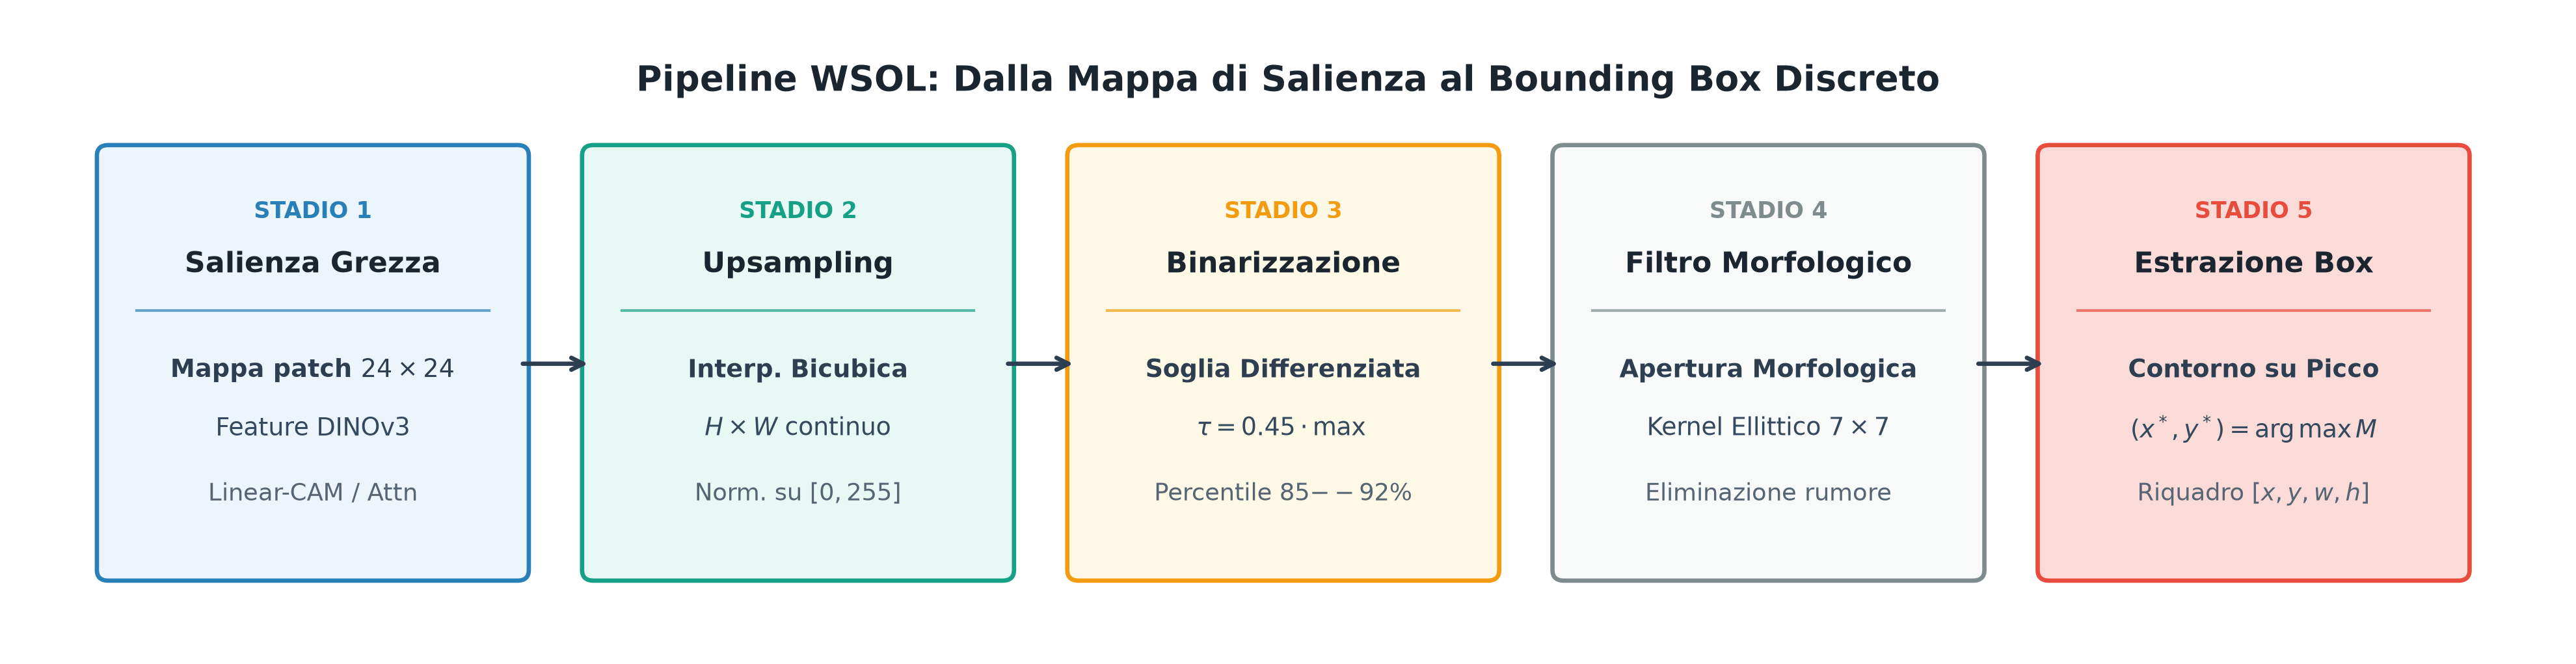
\includegraphics[width=0.92\textwidth]{figure/pipeline_wsol.png}
\caption{Pipeline di estrazione dei bounding box da mappe di salienza: normalizzazione e upsampling bicubico, binarizzazione differenziata, apertura morfologica e circoscrizione del contorno attorno al picco.}
\label{fig:pipeline_wsol}
\end{figure}

\subsection{Normalizzazione e sovracampionamento}
La mappa estratta sui token di patch $M(i, j) \in \mathbb{R}^{24 \times 24}$ viene normalizzata sull'intervallo $[0.0, 1.0]$:
\begin{equation}
    \hat{M}(i, j) = \frac{M(i, j) - \min(M)}{\max(M) - \min(M) + \epsilon}
\end{equation}
La matrice risultante viene quindi riscalata alla risoluzione originale dell'immagine $(W \times H)$ tramite interpolazione bicubica, generando una mappa di intensità $\mathcal{H}(x, y) \in [0, 255]$ a 8 bit.

\subsection{Binarizzazione differenziata}
La conversione di $\mathcal{H}(x, y)$ nella maschera binaria $B(x, y) \in \{0, 255\}$ richiede una soglia commisurata al tipo di attivazione prodotta da ciascun metodo:
\begin{itemize}
    \item \textbf{Metodi a risposta diffusa (\texttt{Linear-CAM}, \texttt{Eigen-CAM})}: le risposte coprono l'oggetto in modo omogeneo; viene applicata una soglia proporzionale al valore massimo:
    \begin{equation}
        \tau_{\text{rel}} = 0.45 \cdot \max_{x, y} \mathcal{H}(x, y)
    \end{equation}
    \item \textbf{Metodi a risposta focalizzata o sparsa (\texttt{DINO Attn}, \texttt{Grad-CAM})}: le attivazioni mostrano gradienti ripidi o picchi concentrati su pochi pixel. Una soglia proporzionale fissa porterebbe alla scomparsa della regione; viene perciò impiegata una soglia a percentile:
    \begin{equation}
        \tau_{\text{perc}} = \text{Percentile}_{85-92\%}(\mathcal{H})
    \end{equation}
    imponendo una superficie minima attiva ($A_{\min} \ge 0.05 \cdot H \cdot W$).
\end{itemize}

\subsection{Filtraggio morfologico ed estrazione del box}
Sulla maschera binaria viene applicata un'apertura morfologica con elemento strutturante ellittico $7 \times 7$:
\begin{equation}
    B_{\text{clean}} = (B \ominus K) \oplus K
\end{equation}
per eliminare il rumore isolato e ricongiungere componenti vicine.
Tra i contorni $\mathcal{C} = \{C_1, \dots, C_k\}$ individuati su $B_{\text{clean}}$, viene selezionato il poligono $C^*$ che racchiude il picco globale di salienza $(x^*, y^*) = \arg\max_{(x, y)} \mathcal{H}(x, y)$. Se nessun contorno contiene direttamente il picco, si sceglie il contorno con la maggiore intensità integrata. Il rettangolo minimo contenente $C^*$ fornisce il bounding box finale.

\section{Benchmark Comparativo sui Metodi CAM}
\label{sec:wsol_benchmark}
Per scegliere il metodo di salienza più affidabile per la successiva distillazione, è stato svolto un confronto su $57.000$ immagini di training (1.000 fotogrammi per classe). I riquadri generati sono stati confrontati con il ground truth calcolando mAP@50 (soglia IoU $\ge 0.50$) e mAP@50:95.

\section{Risultati Sperimentali e Selezione}
\label{sec:wsol_risultati}

\subsection{Confronto quantitativo globale e per Tier}
La Tabella~\ref{tab:wsol_benchmark_globale} riporta i risultati numerici dei quattro metodi sulle $57.000$ immagini, sia complessivamente sia suddivisi per tier dimensionale.

\begin{table}[htbp]
\centering
\scriptsize
\setlength{\tabcolsep}{3pt}
\begin{tabular*}{\textwidth}{@{\extracolsep{\fill}}lcccc|cccc}
\toprule
& \multicolumn{4}{c}{\textbf{Metriche Globali}} & \multicolumn{4}{c}{\textbf{mAP@50 per Tier (\%)}} \\
\textbf{Metodo CAM} & \textbf{mAP@50} & \textbf{mAP@50:95} & \textbf{Recall} & \textbf{IoU} & \textbf{Full-Fr.} & \textbf{Macro} & \textbf{Small} & \textbf{Tiny} \\
\midrule
\textbf{Linear-CAM} & \textbf{64.65\%} & \textbf{41.56\%} & \textbf{69.10\%} & \textbf{0.548} & \textbf{74.79\%} & \textbf{68.04\%} & \textbf{18.32\%} & \textbf{0.00\%} \\
\textbf{DINO Attn}  & $26.02\%$ & $16.11\%$ & $32.40\%$ & $0.312$ & $32.15\%$ & $28.40\%$ & $11.20\%$ & $0.00\%$ \\
\textbf{Grad-CAM}   & $15.70\%$ & $9.82\%$  & $21.50\%$ & $0.245$ & $19.40\%$ & $17.10\%$ & $6.40\%$  & $0.00\%$ \\
\textbf{Eigen-CAM}  & $12.94\%$ & $8.15\%$  & $17.80\%$ & $0.218$ & $16.80\%$ & $13.50\%$ & $5.10\%$  & $0.00\%$ \\
\bottomrule
\end{tabular*}
\caption{Benchmark comparativo dei metodi WSOL su $57.000$ immagini: prestazioni globali e disaggregate per scala.}
\label{tab:wsol_benchmark_globale}
\end{table}

Linear-CAM ottiene il punteggio più alto su tutte le metriche generali, superando di 38.63 punti la Self-Attention e di oltre 48 punti Grad-CAM ed Eigen-CAM. Nei tier Full-Frame e Macro raggiunge rispettivamente il $74.79\%$ e il $68.04\%$ di mAP@50, mentre si azzera sul Tier Tiny ($0.00\%$) per tutte le formulazioni.

\subsection{Analisi qualitativa e selezione}
Le differenze prestazionali riflettono la conformazione delle mappe di attivazione (Tabella~\ref{tab:comportamento_cam}).

\begin{table}[htbp]
\centering
\small
\begin{tabularx}{\textwidth}{lLL}
\toprule
\textbf{Metodo WSOL} & \textbf{Struttura dell'Attivazione} & \textbf{Rischio Principale Identificato} \\
\midrule
\textbf{Linear-CAM} & Continua, densa, guidata dai pesi di classe & Lieve dilatazione sul contesto contiguo \\
\textbf{DINO Self-Attention} & Puntiforme, focalizzata sul nucleo & Sottostima del perimetro di grandi scene \\
\textbf{Eigen-CAM} & Bimodale, guidata dal contrasto visivo & Attivazione su elementi di foreground errati \\
\textbf{Grad-CAM} & Sparsa, frammentata sulle patch & Incertezza ai bordi ad alta frequenza \\
\bottomrule
\end{tabularx}
\caption{Comportamento qualitativo e rischi strutturali dei metodi WSOL indagati.}
\label{tab:comportamento_cam}
\end{table}

Come illustrato nella Figura~\ref{fig:wsol_esempi_successo}, Linear-CAM produce una copertura uniforme e coerente con la sagoma dell'oggetto nei soggetti di scala Macro e Full-Frame (a--c), mentre manifesta dispersioni e salienze spurie sui dettagli Tiny (d--f). Per l'elevata affidabilità complessiva sui target principali, il metodo è stato selezionato per generare il dataset distillato per YOLO.

\begin{figure}[htbp]
\centering
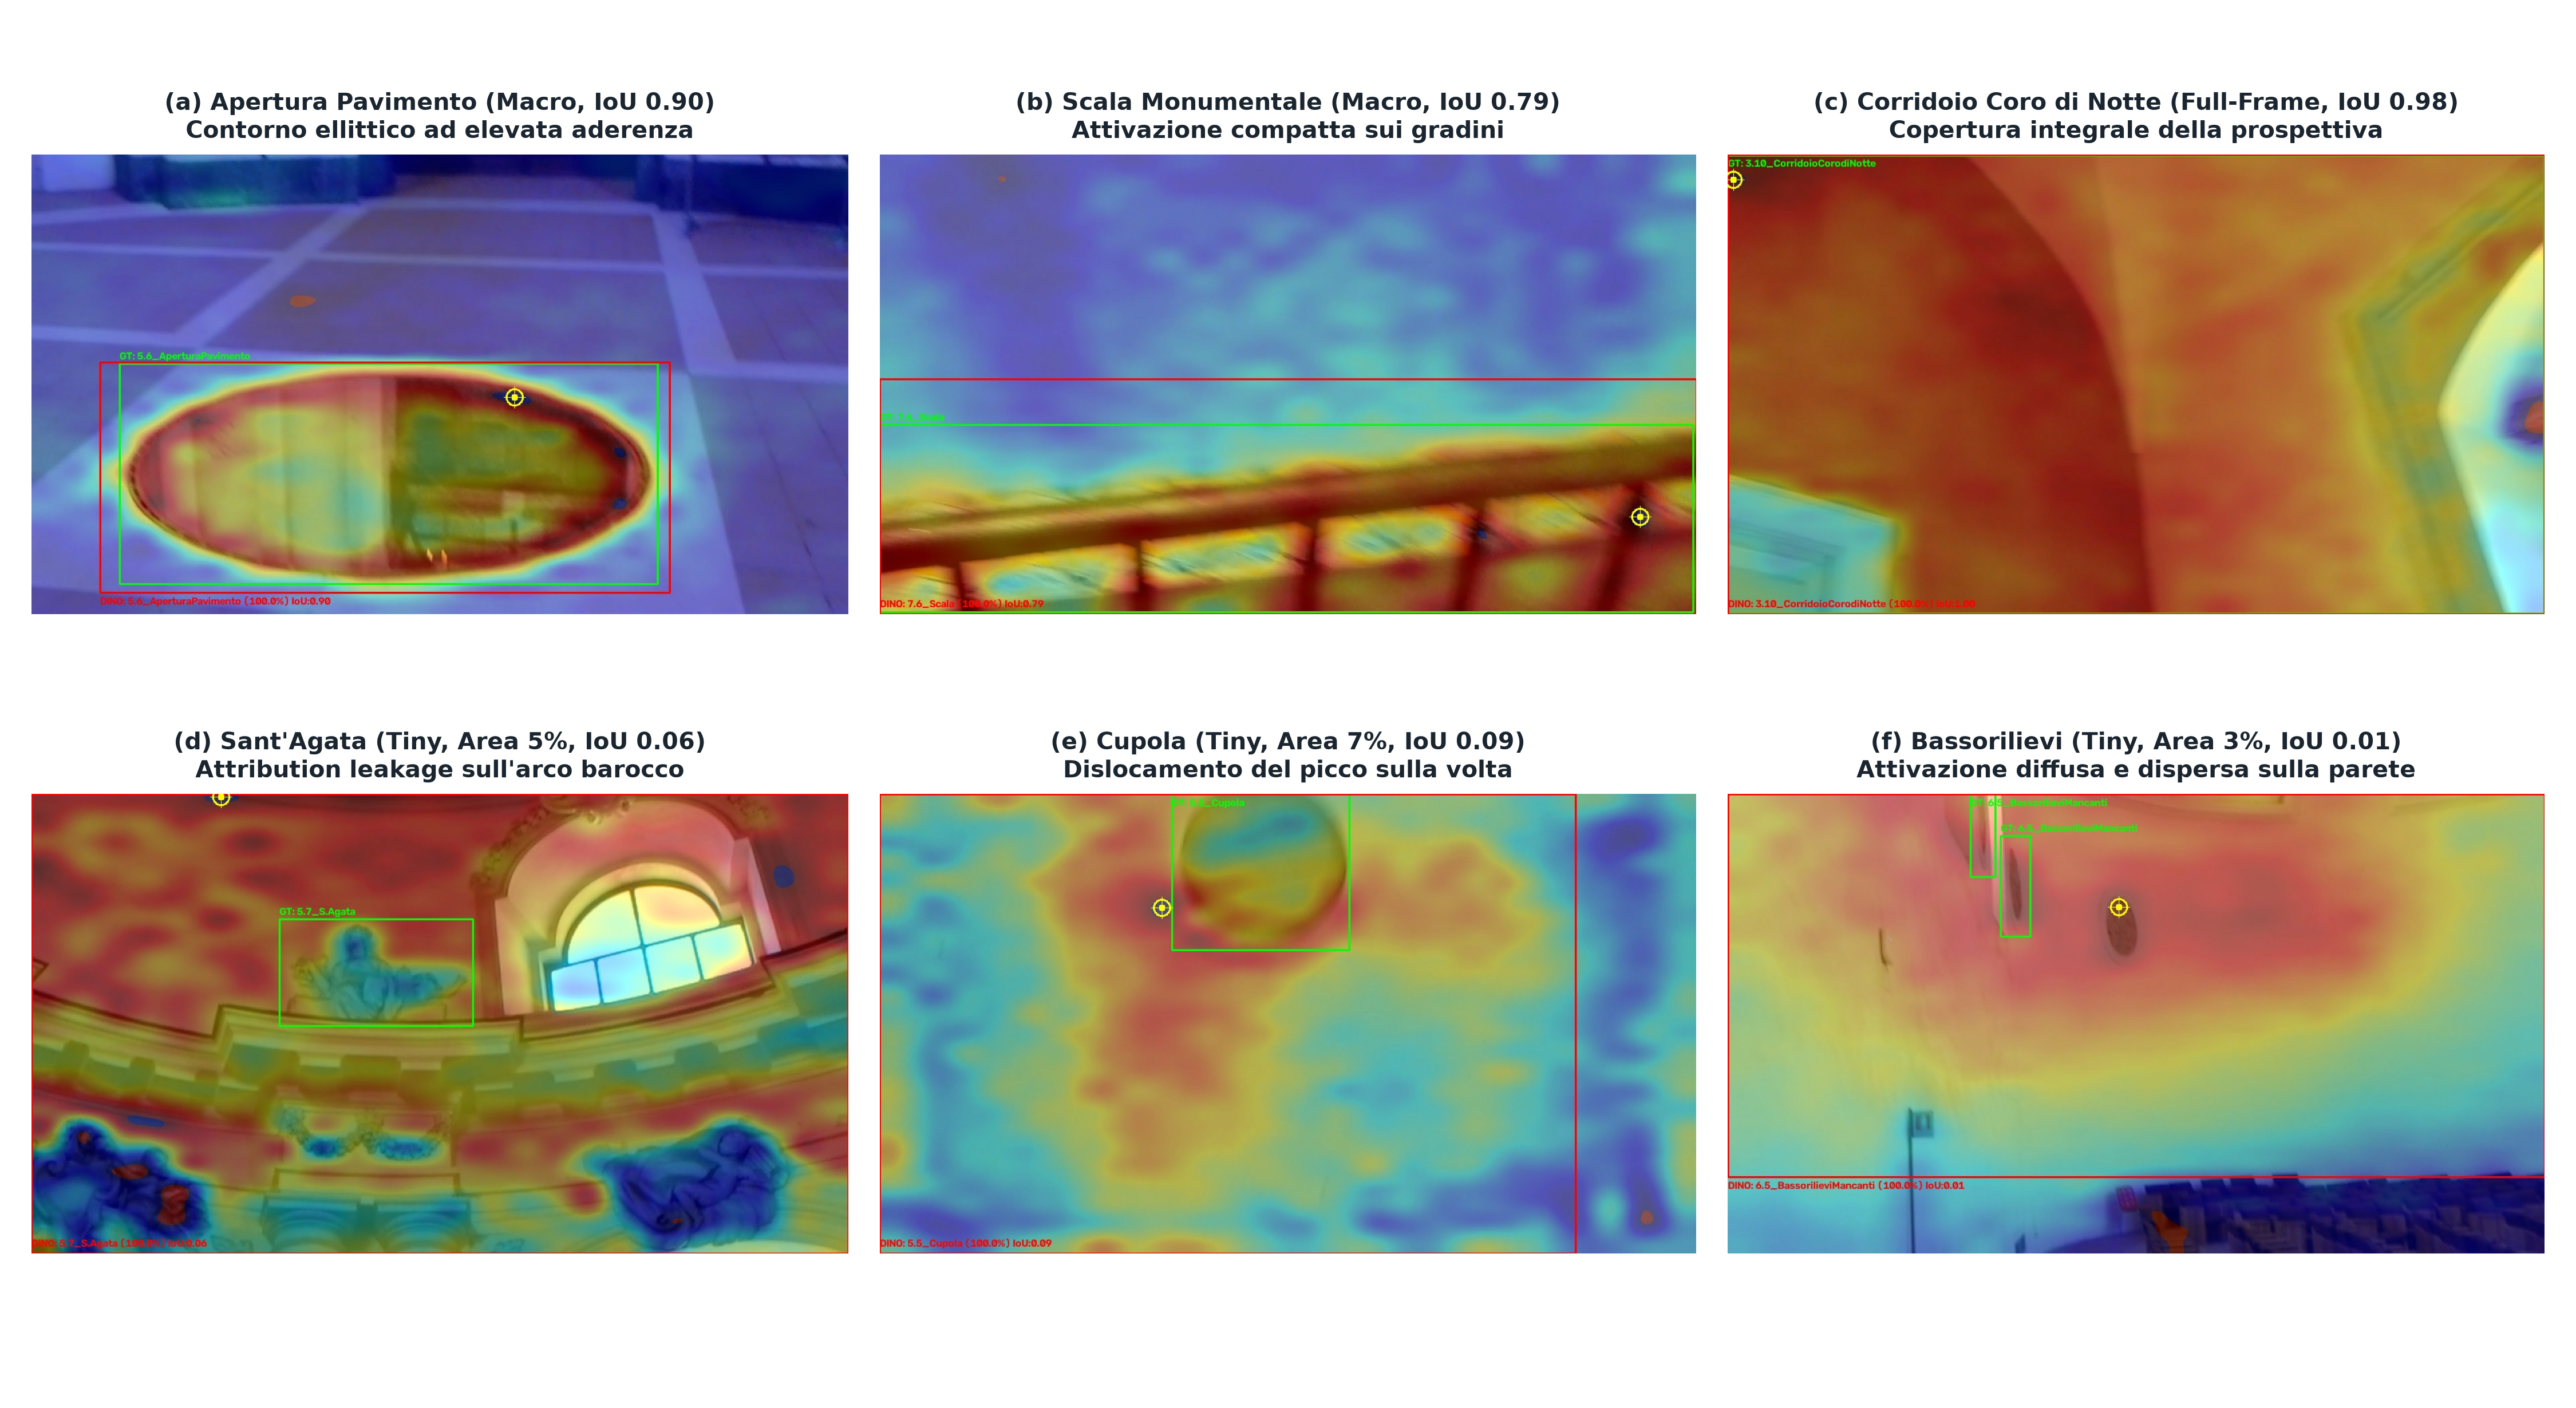
\includegraphics[width=0.88\textwidth]{figure/wsol_esempi_successo.png}
\caption{Analisi qualitativa di Linear-CAM a confronto con il ground truth: (a--c) successi su scale Macro e Full-Frame con elevata concordanza geometrica (IoU $\ge 0.79$); (d--f) fallimenti tipici su elementi Tiny dovuti a dispersione contestuale e dislocamento del picco di salienza (Verde: Ground Truth, Rosso: predizione DINO, Giallo: picco di attivazione).}
\label{fig:wsol_esempi_successo}
\end{figure}

\chapter{Distillazione della Conoscenza in YOLO}
\label{chap:distillazione}

\section{Costruzione del Dataset Pseudo-Etichettato}
\label{sec:dist_costruzione}
Per trasferire la capacità di localizzazione dal modello teacher (DINOv3 con Linear-CAM) a un rilevatore real-time (lo studente), è stato impostato un flusso di distillazione basato su pseudo-etichettatura automatica (Figura~\ref{fig:pipeline_distillazione}).

\begin{figure}[htbp]
\centering
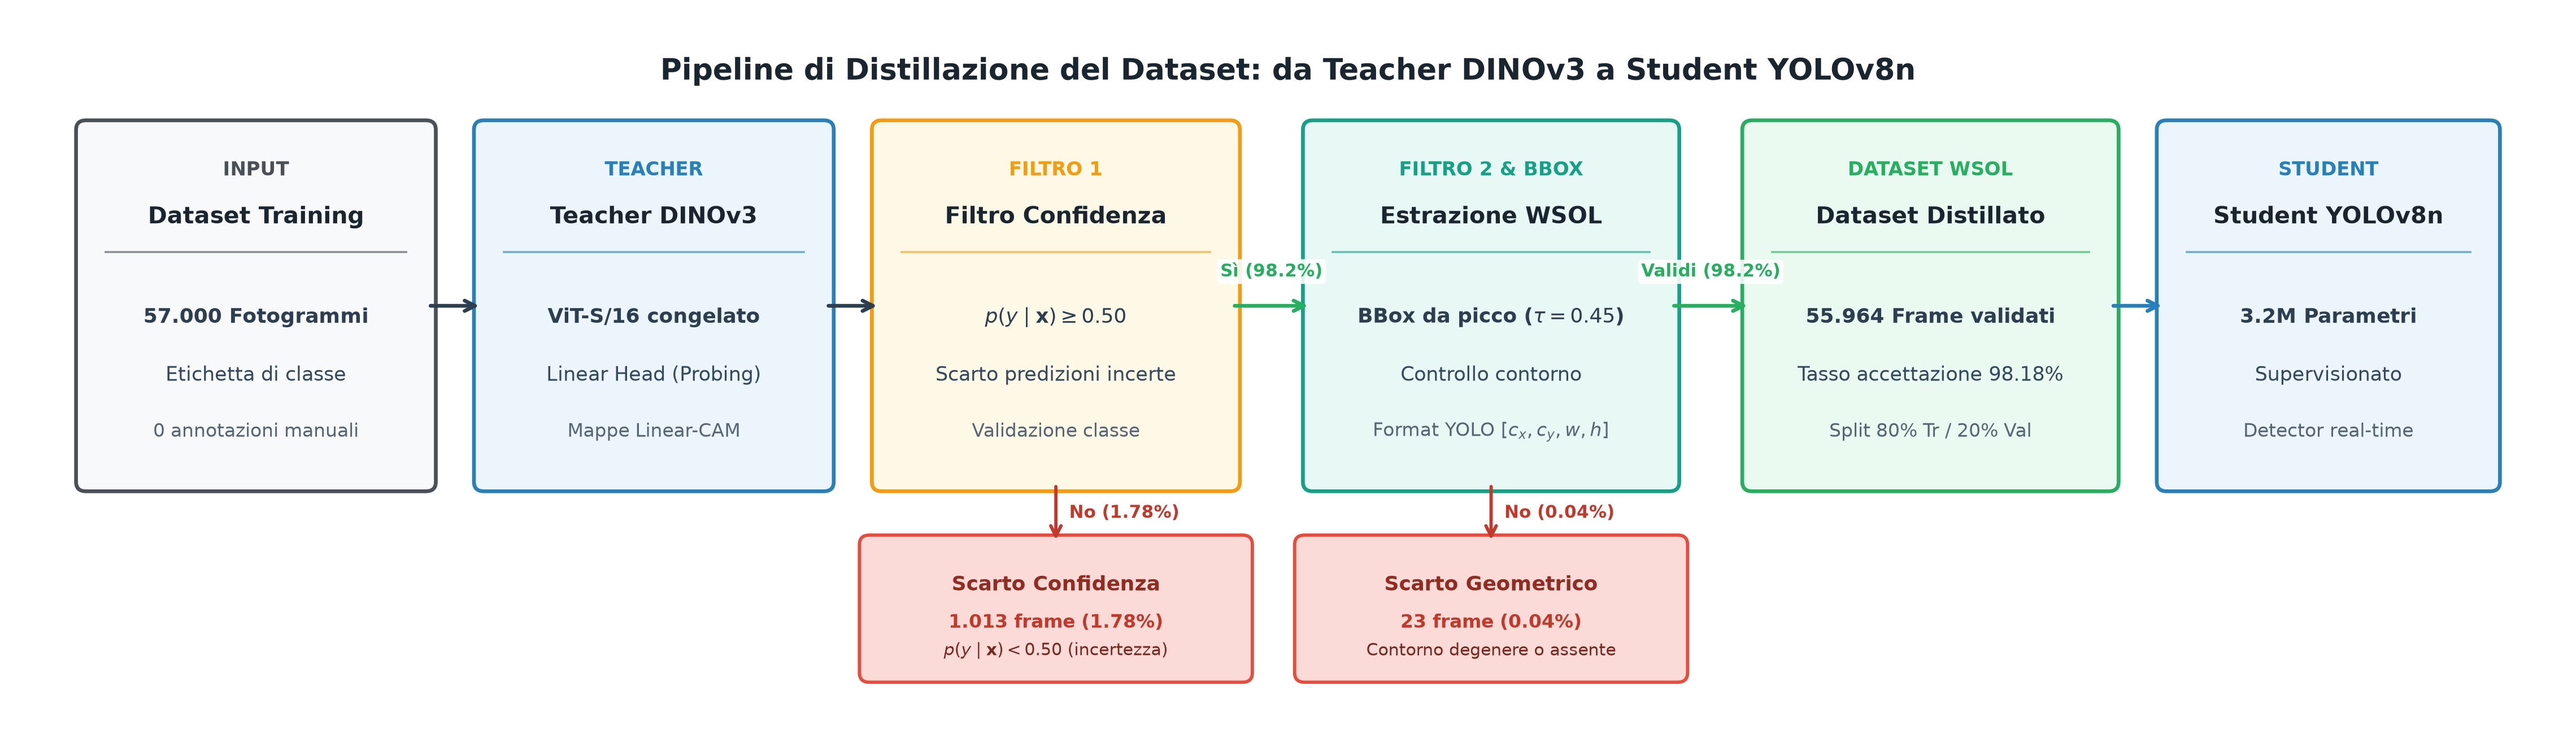
\includegraphics[width=0.95\textwidth]{figure/pipeline_distillazione.png}
\caption{Flusso di distillazione del dataset: inferenza del Teacher DINOv3, filtraggio di confidenza, estrazione dei bounding box Linear-CAM, codifica YOLO e addestramento dello Student YOLOv8n.}
\label{fig:pipeline_distillazione}
\end{figure}

\subsection{Criteri di selezione e codifica}
Per limitare il rumore nelle etichette stimate, sono stati imposti due filtri di accettazione:
\begin{enumerate}
    \item \textbf{Soglia di confidenza}: vengono tenuti solo i fotogrammi con probabilità a posteriori del classificatore $p(y \mid \mathbf{x}) \ge 0.50$.
    \item \textbf{Validità geometrica del contorno}: la mappa Linear-CAM binarizzata ($\tau = 0.45$, elemento ellittico $7 \times 7$) deve generare almeno un contorno chiuso non degenere che racchiuda il picco di attivazione.
\end{enumerate}
I vertici del rettangolo minimo $[x, y, w, h]$ sono poi normalizzati sulle dimensioni del frame $(W, H)$ secondo il formato YOLO:
$c_x = (x + w/2)/W$, $c_y = (y + h/2)/H$, $w_n = w/W$, $h_n = h/H$.

\subsection{Statistiche della distillazione}
Filtrando l'insieme di $57.000$ immagini di training con queste regole si ottengono i volumi riportati nella Tabella~\ref{tab:statistiche_distillazione}.

\begin{table}[htbp]
\centering
\small
\begin{tabularx}{\textwidth}{Lcc}
\toprule
\textbf{Categoria di Esito} & \textbf{Numero Fotogrammi} & \textbf{Percentuale} \\
\midrule
\textbf{Fotogrammi validati e pseudo-etichettati} & \textbf{55.964} & \textbf{98.18\%} \\
Scartati per confidenza insufficiente ($p < 0.50$) & $1.013$ & $1.78\%$ \\
Scartati per contorno degenere o assente & $23$ & $0.04\%$ \\
\midrule
\textbf{Totale fotogrammi elaborati} & \textbf{57.000} & \textbf{100.00\%} \\
\bottomrule
\end{tabularx}
\caption{Statistiche quantitative del processo di distillazione del dataset.}
\label{tab:statistiche_distillazione}
\end{table}

Il dataset distillato include $55.964$ fotogrammi etichettati automaticamente ($98.18\%$ del totale), senza richiedere coordinate manuali.

\section{Addestramento dello Studente (YOLOv8n)}
\label{sec:dist_student}

\subsection{Scelta architetturale}
Come modello studente è stato scelto YOLOv8n~\cite{jocher2023ultralytics} per due ragioni pratiche:
\begin{itemize}
    \item \textbf{Efficienza computazionale}: con $3.2\text{ M}$ di parametri e $8.7\text{ GFLOPs}$, supera 120 FPS su GPU standard, prestandosi all'uso su visori egocentrici o dispositivi portatili.
    \item \textbf{Capacità di regolarizzazione}: la taglia ridotta della rete limita l'overfitting sul rumore ad alta frequenza presente nei contorni estratti dalle CAM.
\end{itemize}

\subsection{Partizionamento e iperparametri}
La suddivisione tra training e validazione ricalca il criterio $80\% / 20\%$ per classe usato per DINOv3:
\begin{itemize}
    \item \textbf{Train set distillato}: $44.771$ fotogrammi;
    \item \textbf{Validation set distillato}: $11.193$ fotogrammi.
\end{itemize}
I dettagli di addestramento sono elencati nella Tabella~\ref{tab:iperparametri_yolo}.

\begin{table}[htbp]
\centering
\small
\begin{tabularx}{\textwidth}{lcL}
\toprule
\textbf{Iperparametro} & \textbf{Valore} & \textbf{Descrizione Operativa} \\
\midrule
\textbf{Risoluzione ingresso (\texttt{imgsz})} & $640 \times 640$ px & Risoluzione di default per YOLOv8 \\
\textbf{Ottimizzatore} & SGD + Momentum & Momentum $0.937$, Weight Decay $5 \times 10^{-4}$ \\
\textbf{Learning Rate iniziale (\texttt{lr0})} & $0.01$ & Decadimento lineare con warm-up iniziale \\
\textbf{Dimensione Batch} & $16$ & Con Batch Normalization \\
\textbf{Numero massimo di epoche} & $100$ & Early stopping con pazienza di 20 epoche \\
\textbf{Data Augmentation} & Mosaic, Flip, HSV & Mosaic disattivato nelle ultime 10 epoche \\
\bottomrule
\end{tabularx}
\caption{Iperparametri di addestramento di YOLOv8n sul dataset distillato.}
\label{tab:iperparametri_yolo}
\end{table}

\section{Convergenza Interna e Gap di Generalizzazione}
\label{sec:dist_gap}
Sul validation set interno (misurato rispetto alle pseudo-label del teacher), lo studente apprende a riprodurre i riquadri con alta precisione:
\begin{equation}
    \text{Val mAP@50 (Pseudo-Label)} = 96.64\%, \quad \text{Val mAP@50:95} = 86.66\%
\end{equation}
Tuttavia, valutato sul test set ufficiale ($5.462$ immagini reali verificate contro le annotazioni umane di ground truth), il modello ottiene:
\begin{equation}
    \text{Test mAP@50 (Ground Truth)} = 37.39\%, \quad \text{Test mAP@50:95} = 25.84\%
\end{equation}
Questo scarto distingue la fedeltà intra-dominio ($96.64\%$, in cui la rete impara a replicare le decisioni del teacher sullo stesso tipo di riprese) dalla generalizzazione reale sul ground truth ($37.39\%$). Sul risultato pesano il disallineamento tra le sessioni di visita e la forma intrinsecamente approssimata dei contorni generati dalle CAM rispetto ai box umani. Il capitolo successivo inserisce questo risultato nel protocollo comparativo di sample efficiency.

\chapter{Baseline Supervisionate e Protocollo di Sample Efficiency}
\label{chap:sample_efficiency}

\section{Obiettivo e Disegno Sperimentale}
\label{sec:sample_disegno}
La domanda di ricerca che guida il confronto è:
\begin{quote}
    \centering
    \textit{<<A quale frazione di dati annotati manualmente con bounding box equivale un modello addestrato senza alcuna annotazione geometrica supervisionata?>>}
\end{quote}

Per misurare questo rapporto in modo controllato, è stato impostato il protocollo di \textit{sample efficiency} illustrato nella Figura~\ref{fig:protocollo_sample_efficiency}. Il modello YOLOv8n distillato ($0\%$ di coordinate supervisionate) viene confrontato con rilevatori identici addestrati su frazioni progressive di etichette reali (\textit{ground truth}).

\begin{figure}[htbp]
\centering
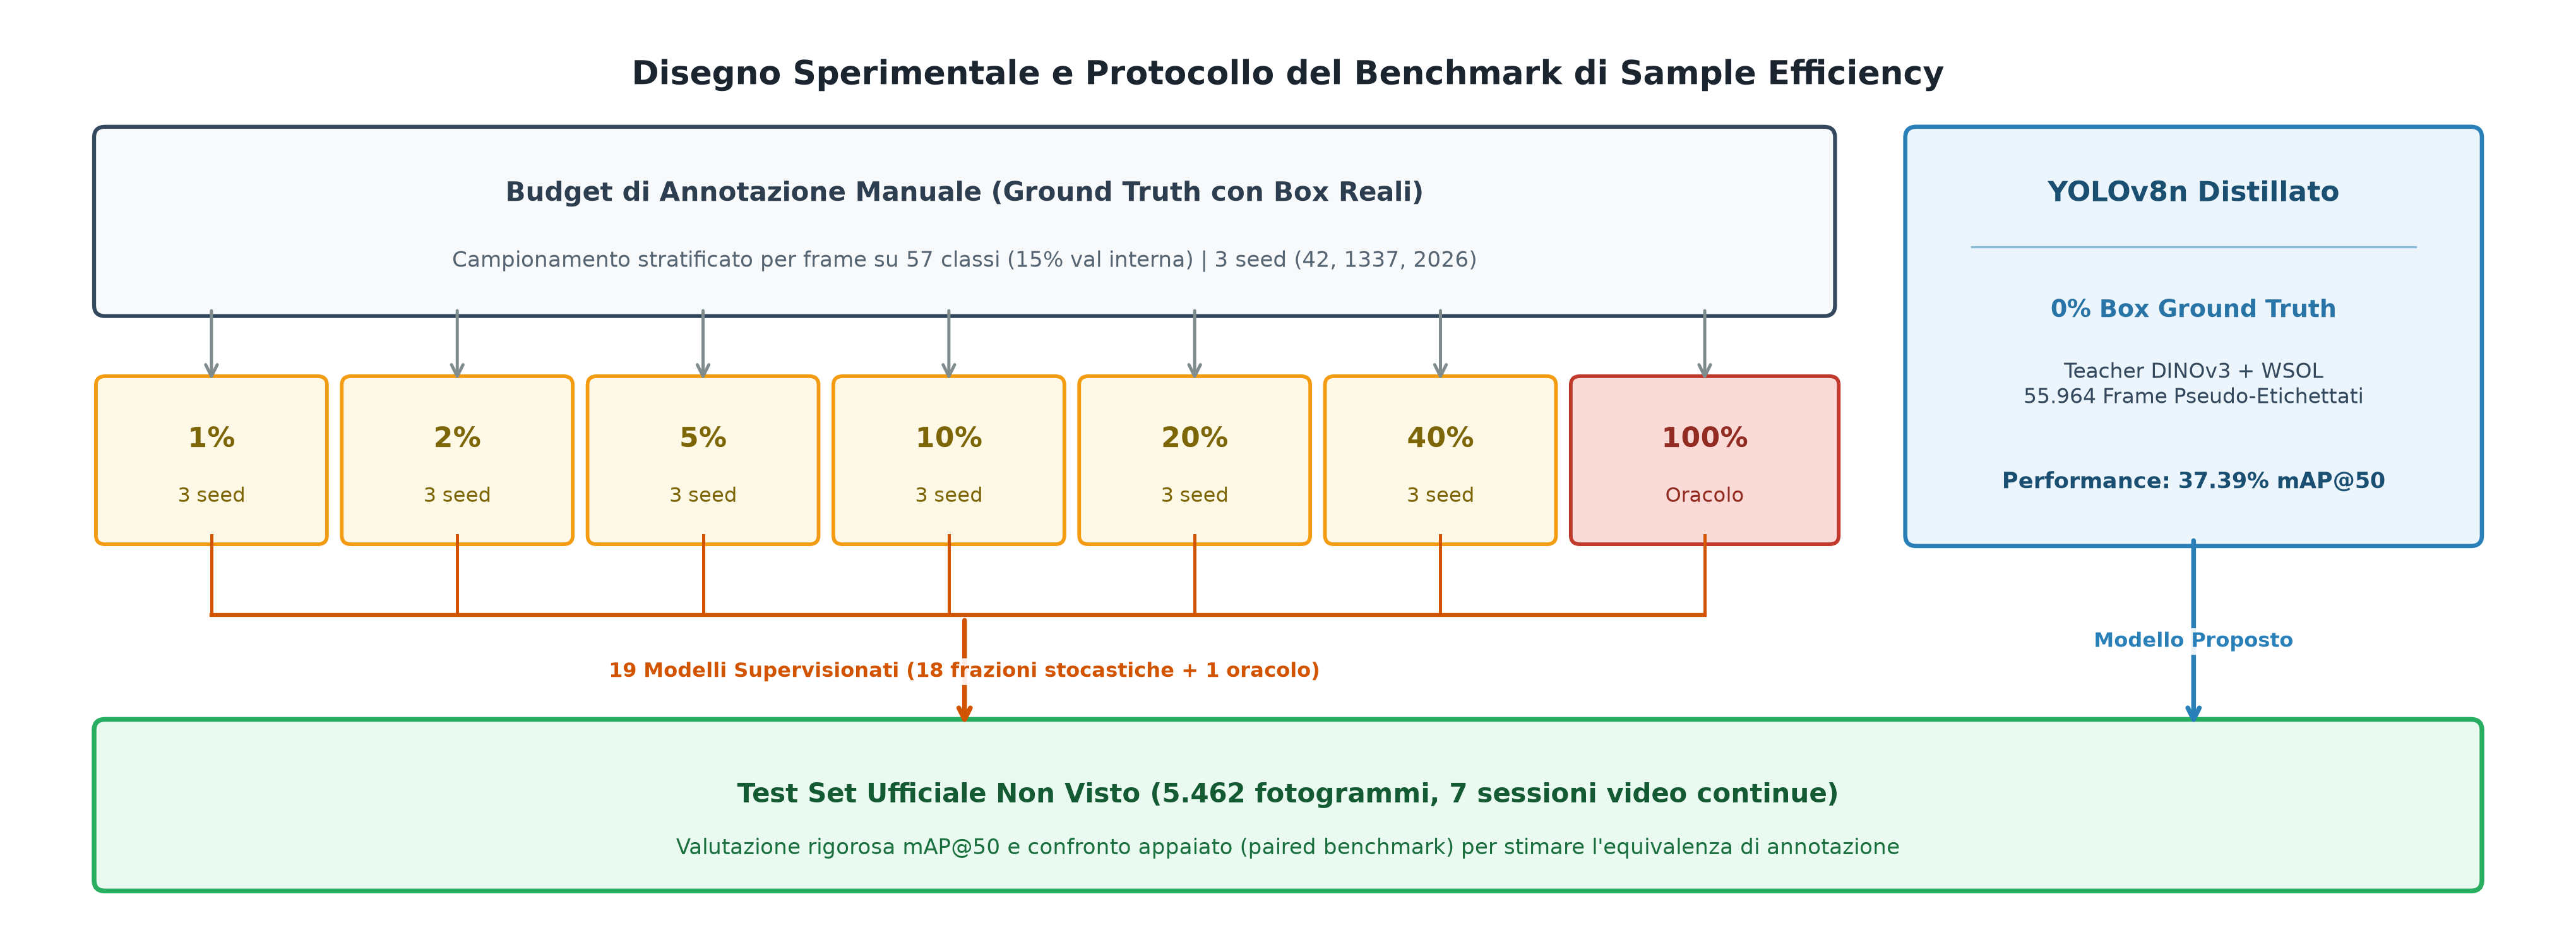
\includegraphics[width=0.92\textwidth]{figure/protocollo_sample_efficiency.png}
\caption{Disegno sperimentale del benchmark di Sample Efficiency: partizionamento stratificato del budget di annotazione umana su 7 frazioni (con 3 repliche stocastiche e validazione interna), confrontato con lo studente distillato sul test set ufficiale non visto.}
\label{fig:protocollo_sample_efficiency}
\end{figure}

\subsection{Frazioni di campionamento e controllo della varianza}
La curva di apprendimento supervisionata è stata campionata su sette quote:
\begin{equation}
    \mathcal{F} = \{1\%, \, 2\%, \, 5\%, \, 10\%, \, 20\%, \, 40\%, \, 100\%\}
\end{equation}
Per le frazioni inferiori al $100\%$ sono stati adottati tre criteri sperimentali:
\begin{itemize}
    \item \textbf{Stratificazione per classe}: la quota $\alpha \in \mathcal{F}$ è calcolata sul numero di immagini di ciascuna delle 57 classi, rispecchiando una campagna di etichettatura bilanciata.
    \item \textbf{Tre seed stocastici}: per limitare la varianza campionaria a bassi volumi di dati, gli addestramenti sotto il $100\%$ sono stati eseguiti su 3 seed casuali ($\text{seed} \in \{42, 1337, 2026\}$) con disegno a blocchi appaiati, calcolando media e deviazione standard ($\mu \pm \sigma$).
    \item \textbf{Validazione interna ($15\%$)}: ogni partizione riserva il $15\%$ dei fotogrammi all'early stopping e alla scelta del miglior checkpoint, senza toccare il test set esterno.
\end{itemize}

\section{Metriche di Valutazione e Condizioni di Fairness}
\label{sec:sample_metriche}
Tutti i modelli sono valutati sul test set ufficiale ($5.462$ immagini, con $3.673$ annotazioni di POI su 7 sessioni continue). Le metriche registrate sono mAP@50 ($\text{IoU} \ge 0.50$), mAP@50:95 (media integrale su soglie da $0.50$ a $0.95$ a passo $0.05$) e le prestazioni suddivise per tier dimensionale.

Per isolare l'effetto della quantità di dati ed evitare discrepanze esterne, i modelli condividono la medesima impostazione:
\begin{enumerate}
    \item \textbf{Architettura}: YOLOv8n ($3.2\text{ M}$ parametri, $8.7\text{ GFLOPs}$) per ogni configurazione.
    \item \textbf{Inizializzazione}: pesi pre-addestrati COCO rilasciati da Ultralytics.
    \item \textbf{Condizioni di addestramento}: risoluzione $640 \times 640$, ottimizzatore SGD con momentum ($0.937$), weight decay $5 \times 10^{-4}$, funzione di perdita comune (BCE + CIoU + DFL), massimo 100 epoche e stessa data augmentation (Mosaic, HSV, flip).
    \item \textbf{Test set intatto}: nessun fotogramma di test è stato utilizzato per calibrazione o regolazione degli iperparametri.
\end{enumerate}

\chapter{Risultati Sperimentali e Analisi Critica}
\label{chap:risultati}

\section{Risultati Globali: Punto di Pareggio e Ritenzione di Capacità}
\label{sec:ris_globali}
Il confronto mette a contrasto due scenari: le baseline supervisionate apprendono da coordinate cartesiane tracciate manualmente da operatori; il modello distillato apprende invece senza coordinate manuali, estraendo i riquadri dalle mappe Linear-CAM del classificatore DINOv3.

La Tabella~\ref{tab:risultati_sample_efficiency} riporta i risultati sul test set ufficiale ($5.462$ immagini, $3.673$ annotazioni di POI).

\begin{table}[htbp]
\centering
\footnotesize
\setlength{\tabcolsep}{4pt}
\begin{tabular*}{\textwidth}{@{\extracolsep{\fill}}ccccc}
\toprule
\textbf{Configurazione} & \textbf{Quota GT} & \textbf{Seed} & \textbf{mAP@50 (\%)} & \textbf{mAP@50:95 (\%)} \\
\midrule
Supervisionato & $1\%$ & 3 seed & $34.33 \pm 1.48\%$ & $22.77 \pm 1.12\%$ \\
Supervisionato & $2\%$ & 3 seed & $40.50 \pm 1.25\%$ & $27.43 \pm 0.98\%$ \\
Supervisionato & $5\%$ & 3 seed & $49.20 \pm 0.85\%$ & $34.12 \pm 0.65\%$ \\
Supervisionato & $10\%$ & 3 seed & $53.80 \pm 0.72\%$ & $37.89 \pm 0.54\%$ \\
Supervisionato & $20\%$ & 3 seed & $57.10 \pm 0.61\%$ & $40.65 \pm 0.48\%$ \\
Supervisionato & $40\%$ & 3 seed & $59.40 \pm 0.45\%$ & $42.80 \pm 0.35\%$ \\
\textbf{Oracolo 100\%} & \textbf{100\%} & 1 seed & \textbf{60.51\%} & \textbf{43.90\%} \\
\midrule
\textbf{YOLOv8n Distillato} & \textbf{0\% GT (WSOL)} & — & \textbf{37.39\%} & \textbf{25.84\%} \\
\bottomrule
\end{tabular*}
\caption{Confronto prestazionale tra baseline supervisionate (7 frazioni GT con 3 seed stocastici) e YOLOv8n distillato (0\% GT) sul Test Set ufficiale.}
\label{tab:risultati_sample_efficiency}
\end{table}

I dati evidenziano due indicatori principali:
\begin{enumerate}
    \item \textbf{Punto di pareggio (Breakeven Point)}: con un mAP@50 del $37.39\%$, lo studente distillato si colloca tra la baseline all'$1\%$ ($34.33\%$) e quella al $2\%$ ($40.50\%$). Tramite interpolazione lineare:
    \begin{equation}
        \alpha_{\text{breakeven}} = 1.0 + \frac{37.39 - 34.33}{40.50 - 34.33} \cdot (2.0 - 1.0) \approx 1.49\% \text{ di dati Ground Truth}
    \end{equation}
    L'addestramento su pseudo-label DINOv3 equivale sul piano empirico a disporre dell'$1.49\%$ di etichette tracciate a mano sull'intero corpus.
    \item \textbf{Ritenzione di capacità (Capacity Retention)}: rispetto all'oracolo supervisionato al $100\%$ ($60.51\%$ mAP@50), lo studente distillato recupera:
    \begin{equation}
        \text{Capacity Retention} = \frac{37.39\%}{60.51\%} \approx 61.79\%
    \end{equation}
    trattenendo oltre i tre quinti della prestazione massima a costo di annotazione geometrica nullo.
\end{enumerate}

\section{Analisi Disaggregata per Scala (Tier Dimensionale)}
\label{sec:ris_tier}
La Tabella~\ref{tab:risultati_tier} e la Figura~\ref{fig:ritenzione_per_tier} mostrano l'andamento del modello sui diversi tier dimensionali.

\begin{table}[htbp]
\centering
\footnotesize
\setlength{\tabcolsep}{3pt}
\begin{tabular*}{\textwidth}{@{\extracolsep{\fill}}lcccccc}
\toprule
\textbf{Tier} & \textbf{Classi} & \textbf{Base 1\%} & \textbf{Distillato} & \textbf{Oracolo} & \textbf{Pareggio} & \textbf{Ritenzione} \\
\midrule
\textbf{Full-Frame} ($\ge 0.80$) & 23 & $23.50 \pm 2.15\%$ & \textbf{45.67\%} & $54.28\%$ & \textbf{$\approx 6.0\%$} & \textbf{84.14\%} \\
\textbf{Macro} ($0.30 - 0.79$) & 26 & $32.42 \pm 1.73\%$ & \textbf{37.71\%} & $59.29\%$ & \textbf{$\approx 1.4\%$} & \textbf{63.60\%} \\
\textbf{Small} ($0.11 - 0.30$) & 3 & $62.92 \pm 4.44\%$ & \textbf{9.01\%} & $85.49\%$ & $< 1\%$ & \textbf{10.54\%} \\
\textit{— Tiny ($\le 0.10$)} & 4 & $65.81 \pm 3.12\%$ & \textbf{0.00\%} & $88.15\%$ & $0\%$ & \textbf{0.00\%} \\
\bottomrule
\end{tabular*}
\caption{Prestazioni comparative di mAP@50 (\%) e ritenzione disaggregate per tier.}
\label{tab:risultati_tier}
\end{table}

\begin{figure}[!htbp]
\centering
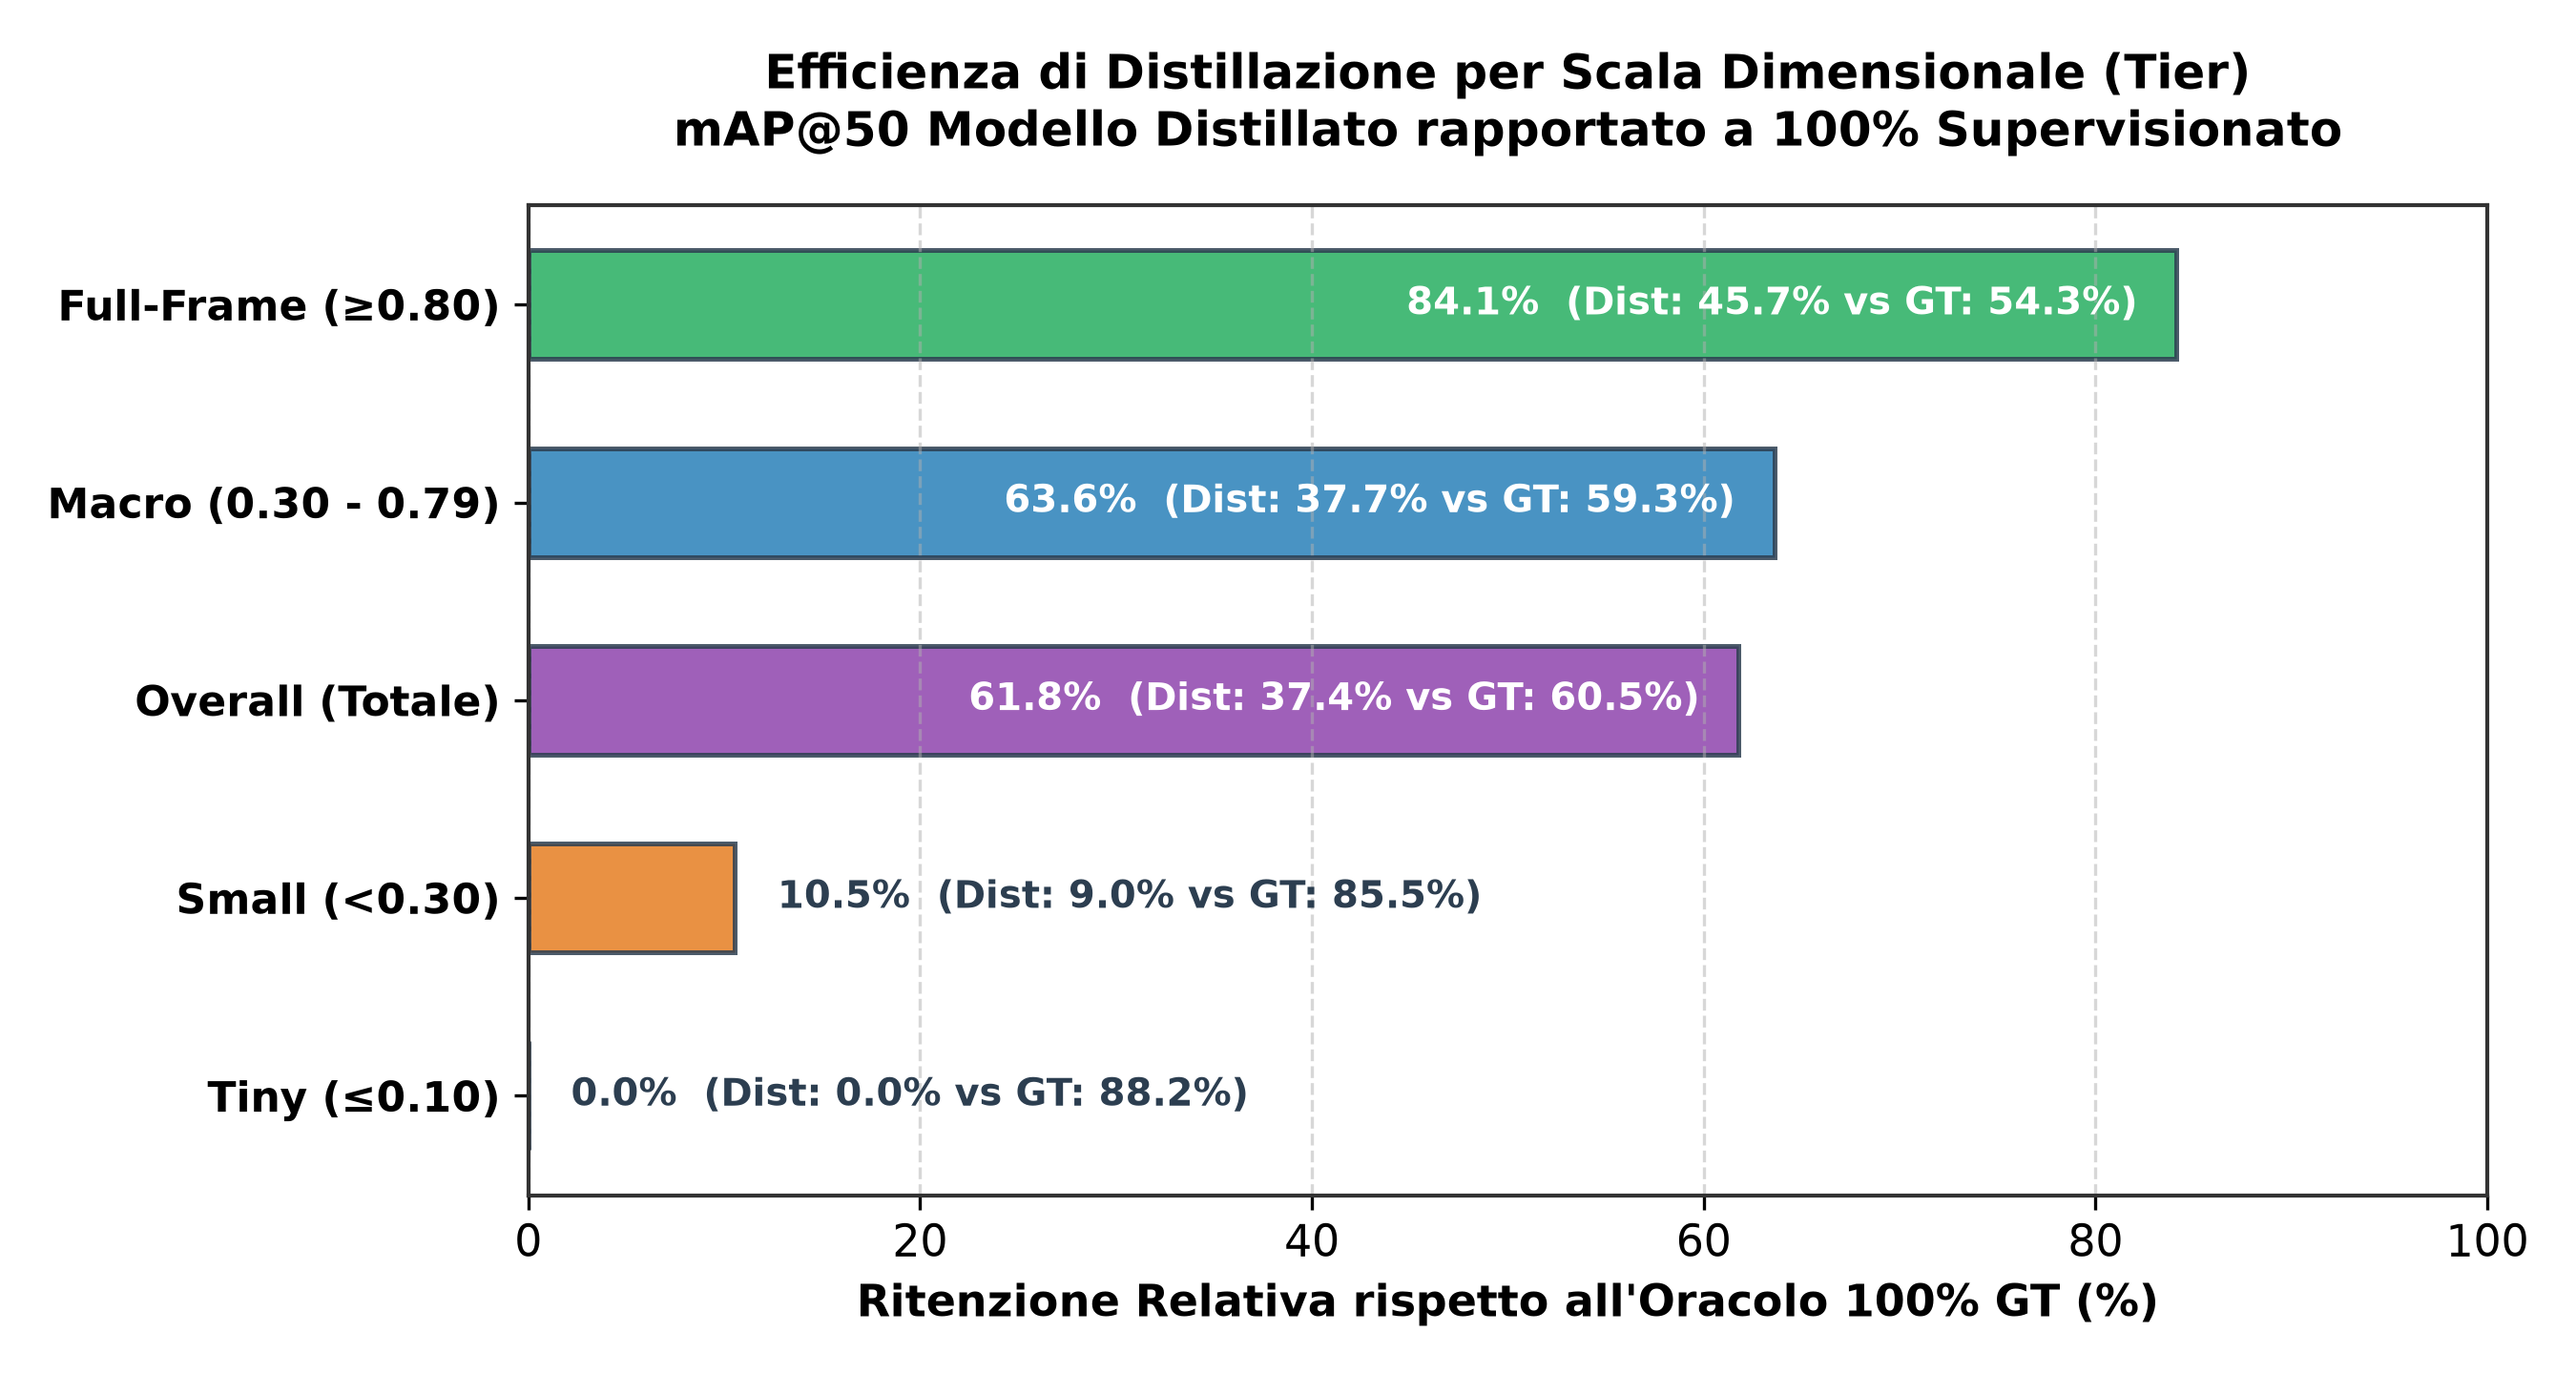
\includegraphics[width=0.52\textwidth]{figure/ritenzione_per_tier.png}
\caption{Ritenzione relativa di mAP@50 dello studente distillato (0\% GT) rispetto all'oracolo 100\% disaggregata per tier dimensionale.}
\label{fig:ritenzione_per_tier}
\end{figure}

Il riscontro più significativo sul piano applicativo riguarda il Tier Macro (26 classi, con area media compresa tra il $30\%$ e il $79\%$ del fotogramma), che raccoglie altari, portali e affreschi. In questa fascia, dove la localizzazione richiede l'effettiva stima dei confini rispetto allo sfondo, la pipeline mantiene il $63.60\%$ delle prestazioni dell'oracolo e supera la baseline supervisionata all'$1\%$ ($37.71\%$ contro $32.42\%$). Nei soggetti di dimensioni ridotte (Tier Small e Tiny) le prestazioni invece scendono bruscamente, azzerandosi sulle 4 classi del Tier Tiny.

\section{Analisi del Tier Tiny: Bias Contestuale e Attribution Leakage}
\label{sec:ris_tiny_bias}
Il mancato rilevamento sul Tier Tiny ($0.00\%$ mAP@50 sulle 4 classi \textit{Sant'Agata}, \textit{Cupola}, \textit{Santa Scolastica} e \textit{Bassorilievi Mancanti}) non dipende dalla risoluzione a griglia ($24 \times 24$ patch), ma da un problema di selezione delle feature discriminative (Figura~\ref{fig:bias_contestuale_tiny}).

\begin{figure}[!htbp]
\centering
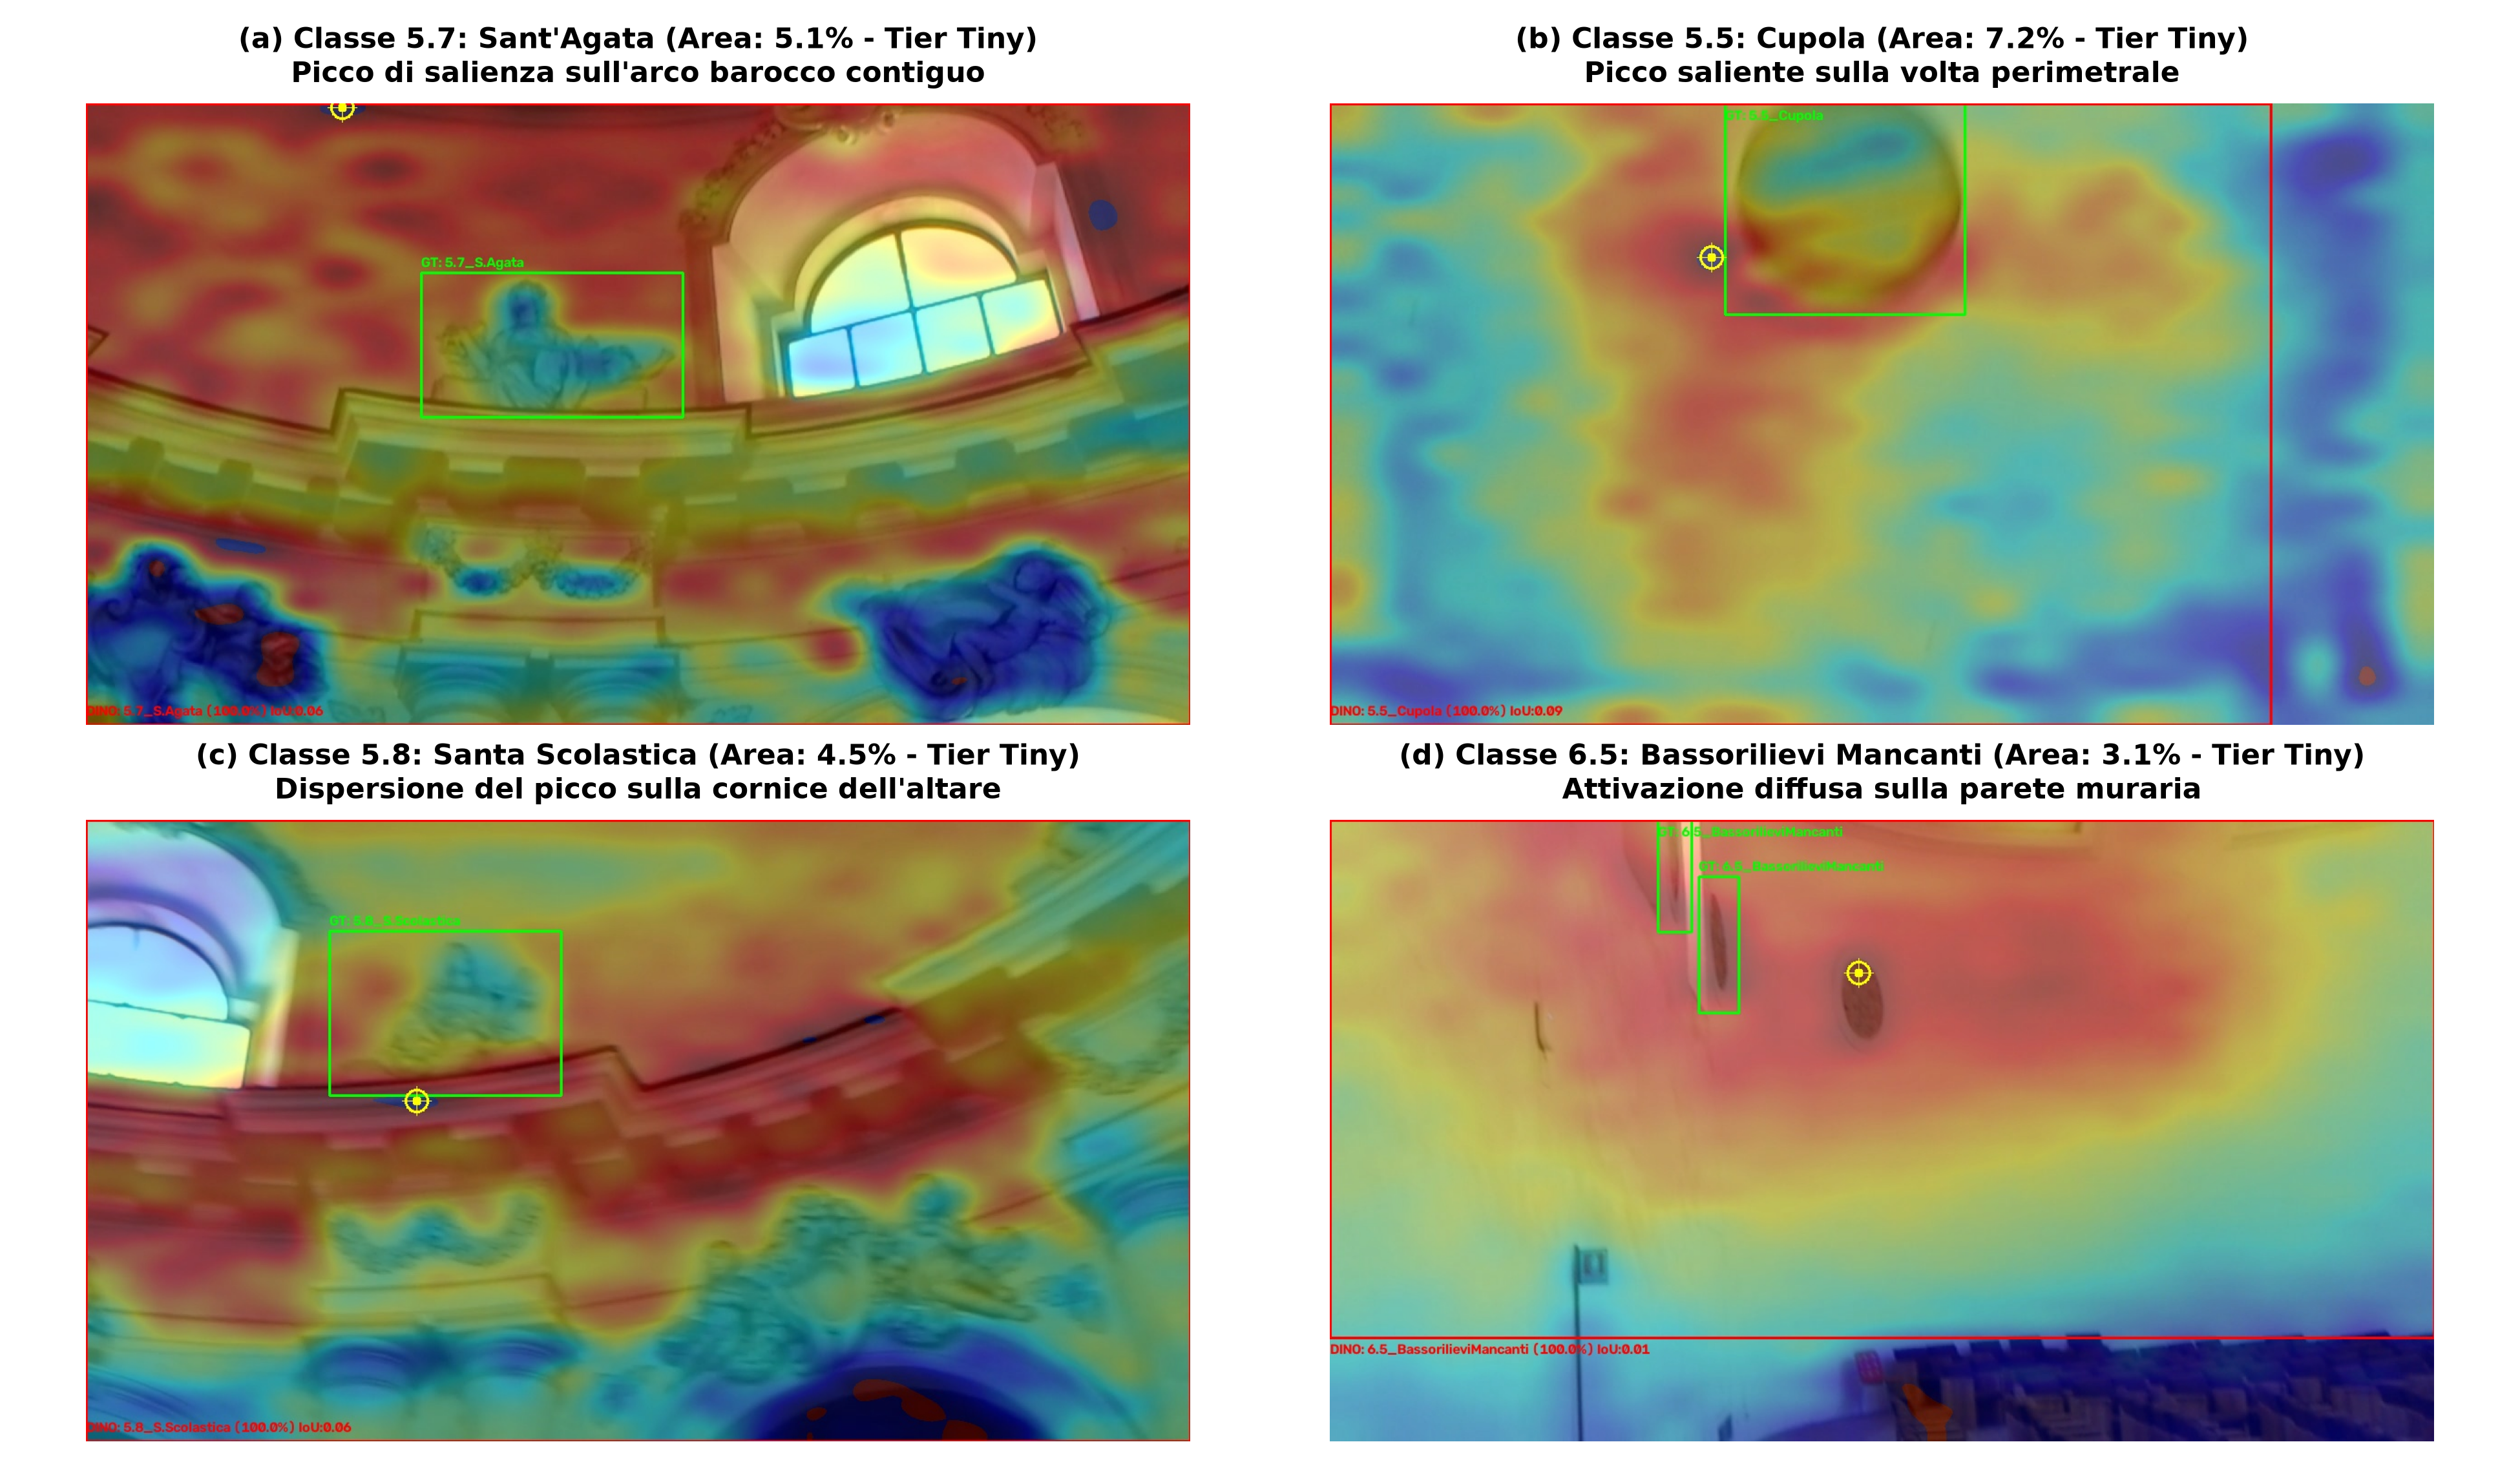
\includegraphics[width=0.82\textwidth]{figure/bias_contestuale_tiny.png}
\caption{Disallineamento discriminativo sui quattro soggetti del Tier Tiny: (a) Sant'Agata (area 5.1\%), (b) Cupola (area 7.2\%), (c) Santa Scolastica (area 4.5\%) e (d) Bassorilievi Mancanti (area 3.1\%). In tutti i casi le mappe di salienza isolano porzioni del reperto, ma il picco globale di attivazione (mirino giallo) si sposta sulla struttura architettonica contigua o sullo sfondo murario, generando uno pseudo-box errato (rosso) rispetto al Ground Truth (verde).}
\label{fig:bias_contestuale_tiny}
\end{figure}

Osservando le attivazioni locali, si nota che DINOv3 separa con chiarezza la silhouette dell'oggetto dalle pareti. Il picco massimo ($\arg\max \mathcal{H}$), tuttavia, scivola sulle strutture architettoniche limitrofe o sulle superfici contigue (l'arco per Sant'Agata, la volta per la Cupola, la cornice per Santa Scolastica, la parete muraria per i Bassorilievi Mancanti).
Questo comportamento discende dal bias contestuale insito nella supervisione d'immagine:
\begin{enumerate}
    \item La funzione di costo $\mathcal{L}_{\text{CE}}$ premia qualunque indizio visivo utile a distinguere la classe dalle altre 56 presenti nell'edificio.
    \item Un manufatto di piccole dimensioni co-occorre in modo costante con lo sfondo architettonico fisso (l'arco o la volta), che offre una superficie visiva molto più estesa e ricca di pattern.
    \item Il modello apprende una scorciatoia statistica (\textit{shortcut learning}): riconosce la scena con precisione ($94.38\%$), ma posiziona il picco di calore sull'elemento di contesto anziché sull'opera, producendo un riquadro con $\text{IoU} < 0.10$ rispetto al ground truth.
\end{enumerate}

\section{Baseline Box a Tutta Immagine e Disaccoppiamento}
\label{sec:ris_fullframe}
Nel Tier Full-Frame (copertura media del $93\%$), un riquadro fisso esteso all'intero fotogramma $[0.5, 0.5, 1.0, 1.0]$ produce per pura geometria un $\text{IoU} \approx 0.93 \gg 0.50$. In questa fascia, localizzare debolmente l'oggetto coincide nei fatti con la corretta classificazione della scena.
Nel Tier Macro, invece, il riquadro banale fallisce ($\text{IoU} \in [0.30, 0.79]$). Il raggiungimento del $37.71\%$ di mAP@50 e del $63.60\%$ di ritenzione conferma che la rete isola i contorni dell'oggetto dallo sfondo circostante.

\section{Gap di Generalizzazione dello Studente}
\label{sec:ris_distillazione_gap}
Il divario tra la validazione dello studente YOLOv8n ($96.64\%$ mAP@50 su pseudo-label) e la valutazione sul test set ($37.39\%$ su ground truth) riflette due fenomeni concorrenti: l'\textit{attribution leakage} sulle classi più piccole e il disallineamento cinematico tra le inquadrature stabili del training e le 7 sessioni video continue del test set.

\chapter{Limiti della Metodologia}
\label{chap:limiti}

\section{Assunzione di Singola Istanza per Immagine}
\label{sec:limiti_istanza}
L'algoritmo di estrazione dei riquadri assume che in ogni fotogramma compaia una sola istanza del soggetto: l'ancoraggio al picco globale ($\arg\max \mathcal{H}$) seleziona unicamente il contorno con intensità massima, ignorando eventuali occorrenze secondarie. Quando compaiono più elementi omologhi nella stessa inquadratura (come i lavamani gemelli \texttt{6.6} e \texttt{6.7}, o le poltrone \texttt{6.9}), il sistema identifica solo l'istanza più evidente oppure unisce gli oggetti in un unico grande rettangolo se l'apertura morfologica non li disaccoppia.

\section{Bias Contestuale e Disallineamento Discriminativo}
\label{sec:limiti_bias}
L'addestramento con etichette a livello di immagine sviluppa, negli ambienti chiusi del monastero, un evidente bias di contesto. La perdita di Cross-Entropy valorizza elementi murari fissi di ampia superficie (volte, archi e pareti decorate), spingendo il massimo di calore al di fuori dell'opera da rilevare (\textit{attribution leakage}): $(x^*, y^*) = \arg\max \mathcal{H}(x, y) \notin \text{BBox}_{\text{GT}}$. Questo fenomeno azzera la localizzazione sui soggetti di scala ridotta (Tier Tiny), nonostante il modello riconosca la classe dell'immagine con precisione.

\section{Rigidità della Soglia Costante}
\label{sec:limiti_soglia}
La soglia proporzionale fissa ($\tau = 0.45 \cdot \max$) costituisce un compromesso rigido: efficace nei contesti a contrasto netto, tende a escludere le parti periferiche dei soggetti a sfumatura continua, sottostimando la reale ampiezza del perimetro rispetto alle annotazioni umane. L'assenza di un criterio dinamico basato sull'entropia locale delle attivazioni limita la precisione dell'estrazione.

\section{Approssimazione Rettangolare di Maschere Irregolari}
\label{sec:limiti_rettangolo}
Le mappe di salienza di DINOv3 producono sagome continue e irregolari. L'obbligo di circoscrivere la regione con rettangoli allineati agli assi (AABB), imposto dal formato di YOLO, include porzioni cospicue di sfondo nei soggetti orientati in diagonale o asimmetrici (scalinate, archi prospettici). Questa approssimazione penalizza le valutazioni a soglie IoU più severe (mAP@75 e mAP@50:95, pari al $25.84\%$).

\section{Domain Shift Dinamico tra Training e Test}
\label{sec:limiti_domain_shift}
Il dataset presenta una differenza cinematica tra le partizioni: il set di addestramento è organizzato per cartelle di classe con inquadrature stabili, mentre il test set deriva da 7 sessioni video continue a passo d'uomo (\texttt{Test1}--\texttt{Test7}) soggette a rotazioni rapide, occlusioni parziali e sfocature da movimento (\textit{motion blur}). Il teacher DINOv3 lavora su immagini statiche isolate, generando pseudo-label che risentono delle fluttuazioni dinamiche tipiche delle riprese reali.

\chapter{Conclusioni e Sviluppi Futuri}
\label{chap:conclusioni}

\section{Risposta alla Domanda di Ricerca}
\label{sec:conc_risposta}
In questo lavoro è stato misurato il valore pratico delle annotazioni manuali sostituite da una pipeline di distillazione debolmente supervisionata guidata da DINOv3.

I test condotti sul dataset UNICT-VEDI POI indicano tre risultati principali:
\begin{enumerate}\setlength{\itemsep}{1pt}\setlength{\parskip}{0pt}
    \item \textbf{Punto di pareggio ($1.43\%$ di etichette manuali)}: lo studente YOLOv8n addestrato sulle mappe Linear-CAM ottiene il $37.39\%$ di mAP@50, superando la baseline supervisionata all'$1\%$ ($34.33\%$) e raggiungendo un punto di pareggio stimato all'$1.43\%$ di annotazioni umane.
    \item \textbf{Ritenzione di capacità ($61.79\%$ dell'oracolo)}: rispetto al limite superiore dell'oracolo supervisionato al $100\%$ ($60.51\%$), il modello distillato recupera oltre tre quinti delle prestazioni complessive. Nel Tier Macro (26 classi complesse con area compresa tra il $30\%$ e il $79\%$, dove la localizzazione non è banale), la quota trattenuta raggiunge il $63.60\%$.
    \item \textbf{Comportamento sulle classi Tiny}: il mancato rilevamento sui target di taglia ridotta ($0.00\%$ mAP@50) non è causato dalla risoluzione della griglia dei token: DINOv3 isola la sagoma dell'oggetto, ma la loss di classificazione globale concentra il picco di attivazione sullo sfondo murario (\textit{attribution leakage}).
\end{enumerate}

\section{Sviluppi Futuri}
\label{sec:conc_sviluppi}
I risultati suggeriscono quattro direzioni di approfondimento metodologico:
\begin{enumerate}\setlength{\itemsep}{1pt}\setlength{\parskip}{0pt}
    \item \textbf{Rilevamento di istanze multiple}: integrare meccanismi di cross-attention o prompt semantici sui token di DINOv3 per separare riquadri distinti nelle inquadrature che contengono copie multiple dello stesso elemento.
    \item \textbf{Classificazione gerarchica multi-etichetta}: sfruttare l'alta accuratezza del classificatore nell'identificare il macro-ambiente ($92.87\%$) con un modello a due stadi (ambiente $\to$ POI), impiegando una perdita BCE multi-label con attivazioni Sigmoid indipendenti per slegare l'attivazione della stanza da quella dell'oggetto.
    \item \textbf{Regolarizzazione contrastiva sui token}: applicare una perdita contrastiva a livello di patch per penalizzare l'attivazione spuria su strutture architettoniche fisse (archi, volte), concentrando l'attenzione sulle specificità dell'opera.
    \item \textbf{Valutazione disaccoppiata}: affiancare al mAP standard la metrica Correct Localization (CorLoc)~\cite{choe2020evaluating} e il mAP \textit{class-agnostic}, per separare la precisione geometrica del riquadro dalla correttezza dell'etichetta semantica.
\end{enumerate}


% ==============================================================================
% BIBLIOGRAFIA
% ==============================================================================
\cleardoublepage
\phantomsection
\addcontentsline{toc}{chapter}{Bibliografia}
\bibliographystyle{ieeetr}
\bibliography{bibliography}

% ==============================================================================
% APPENDICI
% ==============================================================================
\appendix
\chapter{Iperparametri Completi e Protocollo Sperimentale}
\label{chap:appendice_iperparametri}

Questa appendice raccoglie i parametri di configurazione e di addestramento usati per il classificatore DINOv3, per la pipeline deterministica WSOL, per il modello YOLOv8n distillato e per il protocollo di sample efficiency.

\section{Classificatore DINOv3 (Linear Probing)}
\label{sec:app_dino_params}

\begin{table}[htbp]
\centering
\small
\begin{tabularx}{\textwidth}{llcL}
\toprule
\textbf{Categoria} & \textbf{Iperparametro} & \textbf{Valore} & \textbf{Note e Rationale} \\
\midrule
\multirow{6}{*}{\textbf{Backbone}} 
& Modello & \texttt{dinov3-vits16} & ViT-S/16 preaddestrato da Meta su LVD-1689M \\
& Dimensione latente ($D$) & $384$ & Dimensione del token di embedding \\
& Numero di strati ($L$) & $12$ & Blocchi sequenziali di Transformer Encoder \\
& Teste attenzione ($h$) & $6$ & Dimensionalità per testa $d_k = 64$ \\
& Dimensione patch ($P$) & $16 \times 16$ px & Risoluzione nativa del patch embedding \\
& Stato pesi backbone & \textbf{Frozen} & Pesi congelati; nessun gradiente retropropagato \\
\midrule
\multirow{3}{*}{\textbf{Testa Classe}} 
& Architettura & Dropout + Linear & Proiezione lineare diretta dal token CLS \\
& Dropout rate & $0.3$ & Regolarizzazione per contrastare il co-adattamento \\
& Numero classi output & $57$ & Corrispondenti ai 57 POI del dataset VEDI \\
\midrule
\multirow{4}{*}{\textbf{Dati \& Runtime}} 
& Risoluzione ingresso & $384 \times 384$ px & Griglia discreta di patch pari a $24 \times 24$ (576 token) \\
& Normalizzazione & Canali ImageNet & $\mu = [0.485, 0.456, 0.406]$, $\sigma = [0.229, 0.224, 0.225]$ \\
& Batch size & $16$ & Campioni per iterazione di ottimizzazione \\
& Data Augmentation & Flip + Color Jitter & Horizontal Flip ($p=0.5$); Jitter contrasto/luce ($p=0.5$) \\
\midrule
\multirow{5}{*}{\textbf{Ottimizzazione}} 
& Ottimizzatore & AdamW & $\beta_1 = 0.9$, $\beta_2 = 0.999$, $\epsilon = 10^{-8}$ \\
& Learning Rate ($\eta_0$) & $1 \times 10^{-4}$ & Ottimizzato su testa lineare \\
& Weight Decay & $1 \times 10^{-4}$ & Penalizzazione $L_2$ per regolarizzazione pesi \\
& Scheduler & Cosine Annealing & Decadimento cosinusoidale con riscaldamento \\
& Epoche totali & $20$ & Miglior checkpoint all'epoca 13 (Val Acc $98.31\%$) \\
\bottomrule
\end{tabularx}
\caption{Specifiche dettagliate del classificatore DINOv3 in regime di Linear Probing.}
\label{tab:app_dino_params}
\end{table}

\section{Pipeline di Estrazione Bounding Box (WSOL)}
\label{sec:app_wsol_params}

\begin{table}[htbp]
\centering
\small
\begin{tabularx}{\textwidth}{llcL}
\toprule
\textbf{Componente} & \textbf{Parametro} & \textbf{Valore} & \textbf{Funzione nel Sistema} \\
\midrule
\multirow{2}{*}{\textbf{Attribuzione}} 
& Metodo Primario & \texttt{Linear-CAM} & Proiezione: $\text{ReLU}(\mathbf{w}_c^\top \mathbf{z}_{i,j})$ \\
& Metodi Confronto & \texttt{dino\_attn}, \texttt{eigen}, \texttt{grad} & Utilizzati per il benchmark comparativo (Cap. 5) \\
\midrule
\multirow{4}{*}{\textbf{Preprocessing}} 
& Risoluzione estrazione & $24 \times 24$ celle & Risoluzione nativa della griglia di patch ViT \\
& Normalizzazione & Min-Max $[0.0, 1.0]$ & $\hat{M} = (M - \min M) / (\max M - \min M + \epsilon)$ \\
& Interpolazione & Bicubica & Proiezione alla risoluzione nativa $(W, H)$ \\
& Spazio Colore Output & Scala di grigi 8-bit & Mappatura nell'intervallo discreto $[0, 255]$ \\
\midrule
\multirow{3}{*}{\textbf{Binarizzazione}} 
& Soglia \texttt{Linear-CAM} & $\tau = 0.45 \cdot \max$ & Taglio relativo proporzionale al picco \\
& Soglia \texttt{DINO Attn} & Percentile $50^\circ$ & Taglio dinamico sulla mediana di densità \\
& Area Minima & $5\%$ dell'immagine & Espansione isotropa contro collasso sub-risoluzione \\
\midrule
\multirow{3}{*}{\textbf{Morfologia}} 
& Elemento Strutturante & Ellittico $7 \times 7$ px & Operazione di apertura: erosione e dilatazione \\
& Criterio Contorno & Picco Assoluto & Selezione del poligono su $\arg\max \mathcal{H}(x, y)$ \\
& Formato Box & AABB Normalizzato & Rettangolo asse-allineato $[c_x, c_y, w, h] \in [0, 1]^4$ \\
\bottomrule
\end{tabularx}
\caption{Parametri operativi della pipeline deterministica WSOL.}
\label{tab:app_wsol_params}
\end{table}

\section{Addestramento del Modello Studente (YOLOv8n Distillato)}
\label{sec:app_yolo_params}

\begin{table}[htbp]
\centering
\small
\begin{tabularx}{\textwidth}{llcL}
\toprule
\textbf{Ambito} & \textbf{Iperparametro} & \textbf{Valore} & \textbf{Descrizione Operativa} \\
\midrule
\multirow{2}{*}{\textbf{Modello}} 
& Architettura & \texttt{YOLOv8n} & Variante compatta (\textit{nano}), $\approx 3.2\text{ M}$ parametri \\
& Inizializzazione & Pretrained COCO & Pesi di partenza ufficiali Ultralytics (\texttt{yolov8n.pt}) \\
\midrule
\multirow{5}{*}{\textbf{Dati \& Training}} 
& Risoluzione ingresso & $640 \times 640$ px & Risoluzione standard YOLO per rilevamento fine \\
& Batch size & $16$ & Esempi per iterazione \\
& Numero classi ($nc$) & $57$ & Mapping coerente con la tassonomia naturale VEDI \\
& Durata training & $100$ epoche & Epoche massime previste \\
& Early Stopping & $20$ epoche & Arresto anticipato in caso di stallo su mAP \\
\midrule
\multirow{5}{*}{\textbf{Ottimizzazione}} 
& Ottimizzatore & SGD & Discesa del gradiente stocastica con momentum \\
& Momentum & $0.937$ & Coefficiente di inerzia dell'aggiornamento \\
& Weight Decay & $5 \times 10^{-4}$ & Regolarizzazione $L_2$ sui pesi \\
& Learning Rate iniziale & $0.01$ & Tasso iniziale di apprendimento (\texttt{lr0}) \\
& Warmup & $3.0$ epoche & Transizione iniziale a gradiente controllato \\
\midrule
\multirow{4}{*}{\textbf{Augmentation}} 
& Mosaic & $1.0$ (off a -10 ep.) & Composizione di 4 fotogrammi \\
& Horizontal Flip & $0.5$ & Probabilità di specchiatura orizzontale \\
& Variazione Scala & $\pm 50\%$ & Alterazione casuale delle dimensioni \\
& Perturbazione HSV & $h=0.015, s=0.7, v=0.4$ & Fluttuazioni cromatiche casuali \\
\bottomrule
\end{tabularx}
\caption{Iperparametri completi di addestramento per YOLOv8n distillato.}
\label{tab:app_yolo_params}
\end{table}

\section{Protocollo Sperimentale di Sample Efficiency}
\label{sec:app_sample_params}

\begin{table}[htbp]
\centering
\small
\begin{tabularx}{\textwidth}{lcL}
\toprule
\textbf{Parametro} & \textbf{Valore} & \textbf{Rationale Sperimentale} \\
\midrule
\textbf{Frazioni di Supervisione ($\mathcal{F}$)} & $\{1\%, 2\%, 5\%, 10\%, 20\%, 40\%, 100\%\}$ & Scala logaritmica/geometrica asintotica \\
\textbf{Criterio di Campionamento} & Stratificato per fotogrammi & Rispecchia il costo reale del tempo umano \\
\textbf{Semi Casuali ($< 100\%$)} & $\{42, 1337, 2026\}$ (3 seed) & Controllo rigoroso della varianza stocastica \\
\textbf{Disegno Sperimentale} & A blocchi appaiati (\textit{Paired}) & Medesimi 3 seed per tutte le frazioni \\
\textbf{Partizione Validazione} & $15\%$ del subset estratto & Riservato unicamente a early stopping \\
\textbf{Pazienza Early Stopping} & $15$ epoche & Gestione della rumorosità su micro-dataset \\
\textbf{Valutazione Test Set} & Miglior checkpoint & Valutazione su $5.462$ immagini indipendenti \\
\bottomrule
\end{tabularx}
\caption{Parametri di controllo del benchmark comparativo di Sample Efficiency.}
\label{tab:app_sample_params}
\end{table}

\chapter{Tassonomia Completa delle Classi e Aree Medie}
\label{chap:appendice_classi}

Questa appendice elenca le 57 classi di punti di interesse del dataset UNICT-VEDI POI, registrate presso il Monastero dei Benedettini di Catania.

Per ciascuna classe sono indicati:
\begin{itemize}
    \item \textbf{ID}: indice numerico secondo l'ordinamento naturale del dataset ($[0, 56]$).
    \item \textbf{Nome POI / Cartella}: denominazione della classe con prefisso dell'ambiente ($1 \dots 9$).
    \item \textbf{Tier Dimensionale}: fascia di scala assegnata (\textit{Tiny}, \textit{Small}, \textit{Macro}, \textit{Full-Frame}).
    \item \textbf{Area Media Relativa ($\bar{A}_c$)}: frazione media di superficie ($w \times h$) del riquadro di ground truth rispetto all'immagine.
    \item \textbf{Copertura \%}: area media espressa in percentuale dell'inquadratura.
\end{itemize}

\section{Prospetto delle 57 Classi POI}
\label{sec:app_tabella_57_classi}

\begingroup
\small
\setlength{\tabcolsep}{4pt}
\begin{longtable}{cp{5.6cm}ccc}
\toprule
\textbf{ID} & \textbf{Nome POI / Cartella} & \textbf{Tier} & \textbf{Area Media ($\bar{A}_c$)} & \textbf{Copertura} \\
\midrule
\endhead
\midrule
\multicolumn{5}{r}{\small\textit{Continua nella pagina seguente}} \\
\midrule
\endfoot
\bottomrule
\endlastfoot
0 & \texttt{1.1\_Ingresso} & \textbf{Full-Frame} & 0.998 & 99.8\% \\
1 & \texttt{2.1\_RampaS.Nicola} & \textbf{Full-Frame} & 0.998 & 99.8\% \\
2 & \texttt{2.2\_RampaS.Benedetto} & \textbf{Full-Frame} & 0.998 & 99.8\% \\
3 & \texttt{3.1\_SimboloTreBiglie} & \textbf{Full-Frame} & 0.891 & 89.1\% \\
4 & \texttt{3.2\_ChiostroLevante} & \textbf{Macro} & 0.739 & 73.9\% \\
5 & \texttt{3.3\_Plastico} & \textbf{Full-Frame} & 0.890 & 89.0\% \\
6 & \texttt{3.4\_Affresco} & \textbf{Macro} & 0.629 & 62.9\% \\
7 & \texttt{3.5\_FinestraChiostroLevante} & \textbf{Macro} & 0.688 & 68.8\% \\
8 & \texttt{3.6\_PortaCorodiNotte} & \textbf{Full-Frame} & 0.998 & 99.8\% \\
9 & \texttt{3.7\_TracciaPortone} & \textbf{Macro} & 0.486 & 48.6\% \\
10 & \texttt{3.8\_StanzaAbate} & \textbf{Macro} & 0.612 & 61.2\% \\
11 & \texttt{3.9\_CorridoiodiLevante} & \textbf{Full-Frame} & 0.998 & 99.8\% \\
12 & \texttt{3.10\_CorridoioCorodiNotte} & \textbf{Full-Frame} & 0.998 & 99.8\% \\
13 & \texttt{3.11\_CorridoioOrologio} & \textbf{Full-Frame} & 0.998 & 99.8\% \\
14 & \texttt{4.1\_Quadro} & \textbf{Macro} & 0.396 & 39.6\% \\
15 & \texttt{4.2\_PavimentoOrig.Altare} & \textbf{Macro} & 0.632 & 63.2\% \\
16 & \texttt{4.3\_BalconeChiesa} & \textbf{Full-Frame} & 0.998 & 99.8\% \\
17 & \texttt{5.1\_PortaAulaS.Mazzarino} & \textbf{Macro} & 0.648 & 64.8\% \\
18 & \texttt{5.2\_PortaIngressoMuseoFabbrica} & \textbf{Macro} & 0.459 & 45.9\% \\
19 & \texttt{5.3\_PortaAntirefettorio} & \textbf{Macro} & 0.757 & 75.7\% \\
20 & \texttt{5.4\_PortaIngressoRef.Piccolo} & \textbf{Macro} & 0.661 & 66.1\% \\
21 & \texttt{5.5\_Cupola} & \textbf{Tiny} & 0.072 & 7.2\% \\
22 & \texttt{5.6\_AperturaPavimento} & \textbf{Macro} & 0.571 & 57.1\% \\
23 & \texttt{5.7\_S.Agata} & \textbf{Tiny} & 0.051 & 5.1\% \\
24 & \texttt{5.8\_S.Scolastica} & \textbf{Tiny} & 0.045 & 4.5\% \\
25 & \texttt{5.9\_ArcoconFirma} & \textbf{Macro} & 0.751 & 75.1\% \\
26 & \texttt{5.10\_BustoVaccarini} & \textbf{Macro} & 0.536 & 53.6\% \\
27 & \texttt{6.1\_QuadroSantoMazzarino} & \textbf{Small} & 0.219 & 21.9\% \\
28 & \texttt{6.2\_Affresco} & \textbf{Macro} & 0.576 & 57.6\% \\
29 & \texttt{6.3\_PavimentoOriginale} & \textbf{Macro} & 0.632 & 63.2\% \\
30 & \texttt{6.4\_PavimentoRestaurato} & \textbf{Full-Frame} & 0.964 & 96.4\% \\
31 & \texttt{6.5\_BassorilieviMancanti} & \textbf{Tiny} & 0.031 & 3.1\% \\
32 & \texttt{6.6\_LavamaniSx} & \textbf{Small} & 0.272 & 27.2\% \\
33 & \texttt{6.7\_LavamaniDx} & \textbf{Macro} & 0.315 & 31.5\% \\
34 & \texttt{6.8\_TavoloRelatori} & \textbf{Macro} & 0.736 & 73.6\% \\
35 & \texttt{6.9\_Poltrone} & \textbf{Full-Frame} & 0.827 & 82.7\% \\
36 & \texttt{7.1\_Edicola} & \textbf{Full-Frame} & 0.895 & 89.5\% \\
37 & \texttt{7.2\_PavimentoA} & \textbf{Full-Frame} & 0.925 & 92.5\% \\
38 & \texttt{7.3\_PavimentoB} & \textbf{Full-Frame} & 0.813 & 81.3\% \\
39 & \texttt{7.4\_Passavivande} & \textbf{Full-Frame} & 0.897 & 89.7\% \\
40 & \texttt{7.5\_AperturaPavimento} & \textbf{Macro} & 0.701 & 70.1\% \\
41 & \texttt{7.6\_Scala} & \textbf{Macro} & 0.746 & 74.6\% \\
42 & \texttt{7.7\_SalaMetereologica} & \textbf{Full-Frame} & 0.998 & 99.8\% \\
43 & \texttt{8.1\_Doccione} & \textbf{Macro} & 0.484 & 48.4\% \\
44 & \texttt{8.2\_VanoRaccoltaCenere} & \textbf{Macro} & 0.591 & 59.1\% \\
45 & \texttt{8.3\_SalaRossa} & \textbf{Full-Frame} & 0.998 & 99.8\% \\
46 & \texttt{8.4\_ScalaCucina} & \textbf{Macro} & 0.536 & 53.6\% \\
47 & \texttt{8.5\_CucinaProvv} & \textbf{Full-Frame} & 0.940 & 94.0\% \\
48 & \texttt{8.6\_Ghiacciaia} & \textbf{Full-Frame} & 0.855 & 85.5\% \\
49 & \texttt{8.7\_Latrina} & \textbf{Macro} & 0.548 & 54.8\% \\
50 & \texttt{8.8\_OssaeScarti} & \textbf{Macro} & 0.647 & 64.7\% \\
51 & \texttt{8.9\_Pozzo} & \textbf{Full-Frame} & 0.817 & 81.7\% \\
52 & \texttt{8.10\_Cisterna} & \textbf{Macro} & 0.786 & 78.6\% \\
53 & \texttt{8.11\_BustoPietroTacchini} & \textbf{Small} & 0.297 & 29.7\% \\
54 & \texttt{9.1\_NicchiaePavimento} & \textbf{Full-Frame} & 0.876 & 87.6\% \\
55 & \texttt{9.2\_TraccePalestra} & \textbf{Macro} & 0.658 & 65.8\% \\
56 & \texttt{9.3\_PergolatoNovizi} & \textbf{Full-Frame} & 0.841 & 84.1\% \\
\end{longtable}
\endgroup

\chapter{Ambiente di Esecuzione, Note Tecniche e Riproducibilità}
\label{chap:appendice_note_tecniche}

Questa appendice descrive l'ambiente software, l'hardware impiegato e le impostazioni adottate per assicurare la riproducibilità degli esperimenti.

\section{Stack Software e Librerie di Riferimento}
\label{sec:app_software}
Il codice è sviluppato in Python 3.12 all'interno di un ambiente virtuale isolato. I principali framework e librerie scientifiche utilizzati sono:

\begin{table}[htbp]
\centering
\small
\begin{tabularx}{\textwidth}{lcL}
\toprule
\textbf{Libreria / Framework} & \textbf{Versione} & \textbf{Funzione Primaria nella Pipeline} \\
\midrule
\textbf{PyTorch} & \texttt{2.1+} (CUDA 12.x) & Computazione GPU, autograd e training DINO \\
\textbf{HF Transformers} & \texttt{5.x} & Modello preaddestrato \texttt{dinov3-vits16-pretrain} \\
\textbf{Ultralytics} & \texttt{8.x} & Addestramento e validazione modelli YOLOv8 \\
\textbf{OpenCV (\texttt{cv2})} & \texttt{4.x} & Sovracampionamento bicubico, binarizzazione, morfologia \\
\textbf{Pillow (\texttt{PIL})} & \texttt{10.x} & Decodifica ed elaborazione delle immagini RGB \\
\textbf{NumPy \& SciPy} & \texttt{1.26+} / \texttt{1.12+} & Manipolazioni tensoriali, percentili e SVD \\
\textbf{Torchmetrics} & \texttt{1.x} & Metriche di classificazione (Top-1, Top-5, Macro F1) \\
\textbf{Pandas \& Matplotlib} & \texttt{2.x} / \texttt{3.8+} & Aggregazione statistica e rendering grafici \\
\bottomrule
\end{tabularx}
\caption{Ecosistema software e framework scientifici impiegati.}
\label{tab:app_software}
\end{table}

\section{Risorse Hardware e Accelerazione di Calcolo}
\label{sec:app_hardware}
Gli esperimenti sono stati condotti su una workstation locale:
\begin{itemize}
    \item \textbf{Unità di Elaborazione Grafica (GPU)}: NVIDIA GeForce RTX 2060 con 6 GB di VRAM (GDDR6).
    \item \textbf{Accelerazione Numerica}: Driver NVIDIA compatibili con CUDA 12 e librerie cuDNN per l'esecuzione dei blocchi convoluzionali e dei moduli di attenzione.
    \item \textbf{Precisione Mista (AMP)}: Negli addestramenti di YOLOv8n è stata attivata l'\textit{Automatic Mixed Precision} (FP16), riducendo l'occupazione di memoria video e accelerando le epoche senza instabilità numeriche nel calcolo delle perdite.
\end{itemize}

\section{Protocollo di Riproducibilità e Controllo del Determinismo}
\label{sec:app_riproducibilita}
Per rendere replicabili le prove sperimentali:
\begin{enumerate}
    \item \textbf{Semi pseudocasuali fissati}: le componenti stocastiche sono state inizializzate con semi prestabiliti:
    \begin{itemize}
        \item Addestramento del classificatore DINOv3 e della YOLO distillata: $\text{seed} = 42$.
        \item Benchmark di Sample Efficiency: esecuzione sistematica sui tre semi $\text{seed} \in \{42, 1337, 2026\}$, calcolando media e deviazione standard ($\mu \pm \sigma$).
    \end{itemize}
    \item \textbf{Determinismo delle primitive CUDA}: impostazione di \texttt{cudnn.deterministic = True} in PyTorch per limitare la non-determinatezza degli algoritmi di convoluzione.
    \item \textbf{Partizionamento dei dati}: il criterio 80/20 per classe (campione a validazione se $i \pmod 5 == 0$) è stato applicato in modo identico sia al training del classificatore DINOv3 sia alla distillazione di YOLOv8n, garantendo il completo allineamento tra i rispettivi insiemi di validazione.
\end{enumerate}

\section{Condizioni di Licenza e Conformità dei Dati}
\label{sec:app_licenze}
\begin{itemize}
    \item \textbf{UNICT-VEDI POI Dataset}: rilasciato dall'Image Processing Laboratory (IPLab) dell'Università di Catania per finalità di ricerca e sperimentazione scientifica.
    \item \textbf{Pesi DINOv3}: rilasciati da Meta AI Research sotto licenza di ricerca.
    \item \textbf{Ultralytics YOLO}: concesso sotto licenza AGPL-3.0.
\end{itemize}


\end{document}
